\documentclass[12pt,]{book}
\usepackage{lmodern}
\usepackage{amssymb,amsmath}
\usepackage{ifxetex,ifluatex}
\usepackage{fixltx2e} % provides \textsubscript
\ifnum 0\ifxetex 1\fi\ifluatex 1\fi=0 % if pdftex
  \usepackage[T1]{fontenc}
  \usepackage[utf8]{inputenc}
\else % if luatex or xelatex
  \ifxetex
    \usepackage{mathspec}
  \else
    \usepackage{fontspec}
  \fi
  \defaultfontfeatures{Ligatures=TeX,Scale=MatchLowercase}
    \setmonofont[Mapping=tex-ansi,Scale=0.7]{Source Code Pro}
\fi
% use upquote if available, for straight quotes in verbatim environments
\IfFileExists{upquote.sty}{\usepackage{upquote}}{}
% use microtype if available
\IfFileExists{microtype.sty}{%
\usepackage{microtype}
\UseMicrotypeSet[protrusion]{basicmath} % disable protrusion for tt fonts
}{}
\usepackage[margin=1in]{geometry}
\usepackage{hyperref}
\hypersetup{unicode=true,
            pdftitle={The Sainsbury Laboratory Summer School 2017},
            pdfborder={0 0 0},
            breaklinks=true}
\urlstyle{same}  % don't use monospace font for urls
\usepackage{natbib}
\bibliographystyle{apalike}
\usepackage{longtable,booktabs}
\usepackage{graphicx,grffile}
\makeatletter
\def\maxwidth{\ifdim\Gin@nat@width>\linewidth\linewidth\else\Gin@nat@width\fi}
\def\maxheight{\ifdim\Gin@nat@height>\textheight\textheight\else\Gin@nat@height\fi}
\makeatother
% Scale images if necessary, so that they will not overflow the page
% margins by default, and it is still possible to overwrite the defaults
% using explicit options in \includegraphics[width, height, ...]{}
\setkeys{Gin}{width=\maxwidth,height=\maxheight,keepaspectratio}
\IfFileExists{parskip.sty}{%
\usepackage{parskip}
}{% else
\setlength{\parindent}{0pt}
\setlength{\parskip}{6pt plus 2pt minus 1pt}
}
\setlength{\emergencystretch}{3em}  % prevent overfull lines
\providecommand{\tightlist}{%
  \setlength{\itemsep}{0pt}\setlength{\parskip}{0pt}}
\setcounter{secnumdepth}{5}
% Redefines (sub)paragraphs to behave more like sections
\ifx\paragraph\undefined\else
\let\oldparagraph\paragraph
\renewcommand{\paragraph}[1]{\oldparagraph{#1}\mbox{}}
\fi
\ifx\subparagraph\undefined\else
\let\oldsubparagraph\subparagraph
\renewcommand{\subparagraph}[1]{\oldsubparagraph{#1}\mbox{}}
\fi

%%% Use protect on footnotes to avoid problems with footnotes in titles
\let\rmarkdownfootnote\footnote%
\def\footnote{\protect\rmarkdownfootnote}

%%% Change title format to be more compact
\usepackage{titling}

% Create subtitle command for use in maketitle
\newcommand{\subtitle}[1]{
  \posttitle{
    \begin{center}\large#1\end{center}
    }
}

\setlength{\droptitle}{-2em}
  \title{The Sainsbury Laboratory Summer School 2017}
  \pretitle{\vspace{\droptitle}\centering\huge}
  \posttitle{\par}
  \author{}
  \preauthor{}\postauthor{}
  \date{}
  \predate{}\postdate{}

\usepackage{booktabs}
\usepackage{amsthm}
\makeatletter
\def\thm@space@setup{%
  \thm@preskip=8pt plus 2pt minus 4pt
  \thm@postskip=\thm@preskip
}
\makeatother
\setmainfont[UprightFeatures={SmallCapsFont=AlegreyaSC-Regular}]{Alegreya}
\renewcommand{\textfraction}{0.05}
\renewcommand{\topfraction}{0.8}
\renewcommand{\bottomfraction}{0.8}
\renewcommand{\floatpagefraction}{0.75}
\let\oldhref\href
\renewcommand{\href}[2]{#2\footnote{\url{#1}}}

\usepackage{amsthm}
\newtheorem{theorem}{Theorem}[chapter]
\newtheorem{lemma}{Lemma}[chapter]
\theoremstyle{definition}
\newtheorem{definition}{Definition}[chapter]
\newtheorem{corollary}{Corollary}[chapter]
\newtheorem{proposition}{Proposition}[chapter]
\theoremstyle{definition}
\newtheorem{example}{Example}[chapter]
\theoremstyle{remark}
\newtheorem*{remark}{Remark}
\begin{document}
\maketitle

{
\setcounter{tocdepth}{1}
\tableofcontents
}
\chapter*{Welcome to The Sainsbury Laboratory Summer School
2017}\label{welcome-to-the-sainsbury-laboratory-summer-school-2017}
\addcontentsline{toc}{chapter}{Welcome to The Sainsbury Laboratory
Summer School 2017}

The last 20 years have provided a sophisticated understanding of how
plants recognise relatively conserved microbial patterns to activate
defence. In recent years DNA sequencing has allowed genomes and
transcriptomes of eukaryotic rusts and mildew pathogens to be studied.
High-throughput imaging advances have made possible the study and
visualisation of intracellular interactions during pathogenesis and
defence.

We will present and teach on these many aspects of plant-microbe
interactions from the fundamental genomic, cellular and molecular
processes to translational activities about how we convert basic
discovery to real world impact.

The TSL Summer School will focus on dynamic and interactive practical
sessions will naturally promote strong interactions between speakers and
participants.

Over the next two weeks we will cover a wide range of topics, including:

\begin{itemize}
\tightlist
\item
  Pathogenomics
\item
  Effectors
\item
  Surface Immunity
\item
  Bioinformatics
\item
  Resistance Proteins
\item
  Cellular Defence
\item
  Proteomics
\item
  Functional Plant Genomics
\item
  Translation to the field
\end{itemize}

We hope that you will find the whole exercise enlightening and
educational and perhaps also a little fun.

\chapter*{Course schedule}\label{course-schedule}
\addcontentsline{toc}{chapter}{Course schedule}

\section*{Monday 31st July}\label{monday-31st-july}
\addcontentsline{toc}{section}{Monday 31st July}

\emph{Introductions}

\begin{longtable}[]{@{}lll@{}}
\toprule
\begin{minipage}[b]{0.09\columnwidth}\raggedright\strut
Time\strut
\end{minipage} & \begin{minipage}[b]{0.38\columnwidth}\raggedright\strut
Activity\strut
\end{minipage} & \begin{minipage}[b]{0.38\columnwidth}\raggedright\strut
Venue\strut
\end{minipage}\tabularnewline
\midrule
\endhead
\begin{minipage}[t]{0.09\columnwidth}\raggedright\strut
1000\strut
\end{minipage} & \begin{minipage}[t]{0.38\columnwidth}\raggedright\strut
Welcome to TSL and housekeeping\strut
\end{minipage} & \begin{minipage}[t]{0.38\columnwidth}\raggedright\strut
\strut
\end{minipage}\tabularnewline
\begin{minipage}[t]{0.09\columnwidth}\raggedright\strut
1015\strut
\end{minipage} & \begin{minipage}[t]{0.38\columnwidth}\raggedright\strut
Introductions by TSL Staff\strut
\end{minipage} & \begin{minipage}[t]{0.38\columnwidth}\raggedright\strut
\strut
\end{minipage}\tabularnewline
\begin{minipage}[t]{0.09\columnwidth}\raggedright\strut
1030\strut
\end{minipage} & \begin{minipage}[t]{0.38\columnwidth}\raggedright\strut
Participant Introductions\strut
\end{minipage} & \begin{minipage}[t]{0.38\columnwidth}\raggedright\strut
\strut
\end{minipage}\tabularnewline
\begin{minipage}[t]{0.09\columnwidth}\raggedright\strut
1100\strut
\end{minipage} & \begin{minipage}[t]{0.38\columnwidth}\raggedright\strut
PEDAGOGICAL LECTURE - Introduction to Plant Microbe Interactions\strut
\end{minipage} & \begin{minipage}[t]{0.38\columnwidth}\raggedright\strut
\strut
\end{minipage}\tabularnewline
\begin{minipage}[t]{0.09\columnwidth}\raggedright\strut
1200\strut
\end{minipage} & \begin{minipage}[t]{0.38\columnwidth}\raggedright\strut
Lunch\strut
\end{minipage} & \begin{minipage}[t]{0.38\columnwidth}\raggedright\strut
NRP Venues\strut
\end{minipage}\tabularnewline
\begin{minipage}[t]{0.09\columnwidth}\raggedright\strut
1300\strut
\end{minipage} & \begin{minipage}[t]{0.38\columnwidth}\raggedright\strut
Poster Session\strut
\end{minipage} & \begin{minipage}[t]{0.38\columnwidth}\raggedright\strut
John Innes Centre Conference Centre\strut
\end{minipage}\tabularnewline
\begin{minipage}[t]{0.09\columnwidth}\raggedright\strut
1500\strut
\end{minipage} & \begin{minipage}[t]{0.38\columnwidth}\raggedright\strut
Tour of The Sainsbury Laboratory and Norwich Research Park\strut
\end{minipage} & \begin{minipage}[t]{0.38\columnwidth}\raggedright\strut
Meet at John Innes Reception\strut
\end{minipage}\tabularnewline
\bottomrule
\end{longtable}

NB All activities will take place in the Training Suite, unless
otherwise stated

\section*{Tuesday 1st August}\label{tuesday-1st-august}
\addcontentsline{toc}{section}{Tuesday 1st August}

\emph{Resistance Proteins. Led by Jonathan Jones}

\begin{longtable}[]{@{}lll@{}}
\toprule
\begin{minipage}[b]{0.09\columnwidth}\raggedright\strut
Time\strut
\end{minipage} & \begin{minipage}[b]{0.39\columnwidth}\raggedright\strut
Activity\strut
\end{minipage} & \begin{minipage}[b]{0.39\columnwidth}\raggedright\strut
Venue\strut
\end{minipage}\tabularnewline
\midrule
\endhead
\begin{minipage}[t]{0.09\columnwidth}\raggedright\strut
930\strut
\end{minipage} & \begin{minipage}[t]{0.39\columnwidth}\raggedright\strut
PEDAGOGICAL LECTURE - Jonathan Jones\strut
\end{minipage} & \begin{minipage}[t]{0.39\columnwidth}\raggedright\strut
\strut
\end{minipage}\tabularnewline
\begin{minipage}[t]{0.09\columnwidth}\raggedright\strut
1100\strut
\end{minipage} & \begin{minipage}[t]{0.39\columnwidth}\raggedright\strut
Tea Break and Discussion\strut
\end{minipage} & \begin{minipage}[t]{0.39\columnwidth}\raggedright\strut
\strut
\end{minipage}\tabularnewline
\begin{minipage}[t]{0.09\columnwidth}\raggedright\strut
1130\strut
\end{minipage} & \begin{minipage}[t]{0.39\columnwidth}\raggedright\strut
Practical Session\strut
\end{minipage} & \begin{minipage}[t]{0.39\columnwidth}\raggedright\strut
\strut
\end{minipage}\tabularnewline
\begin{minipage}[t]{0.09\columnwidth}\raggedright\strut
1230\strut
\end{minipage} & \begin{minipage}[t]{0.39\columnwidth}\raggedright\strut
Lunch\strut
\end{minipage} & \begin{minipage}[t]{0.39\columnwidth}\raggedright\strut
NRP Venues\strut
\end{minipage}\tabularnewline
\begin{minipage}[t]{0.09\columnwidth}\raggedright\strut
1330\strut
\end{minipage} & \begin{minipage}[t]{0.39\columnwidth}\raggedright\strut
KEYNOTE LECTURE - JIJIE CHAI - Structural Study of Plant Receptor
Kinases\strut
\end{minipage} & \begin{minipage}[t]{0.39\columnwidth}\raggedright\strut
Jane Rogers Seminar Room at EI\strut
\end{minipage}\tabularnewline
\begin{minipage}[t]{0.09\columnwidth}\raggedright\strut
1430\strut
\end{minipage} & \begin{minipage}[t]{0.39\columnwidth}\raggedright\strut
Tea Break and Discussion\strut
\end{minipage} & \begin{minipage}[t]{0.39\columnwidth}\raggedright\strut
\strut
\end{minipage}\tabularnewline
\begin{minipage}[t]{0.09\columnwidth}\raggedright\strut
1500\strut
\end{minipage} & \begin{minipage}[t]{0.39\columnwidth}\raggedright\strut
Practical Session\strut
\end{minipage} & \begin{minipage}[t]{0.39\columnwidth}\raggedright\strut
\strut
\end{minipage}\tabularnewline
\bottomrule
\end{longtable}

\section*{Wednesday 2nd August}\label{wednesday-2nd-august}
\addcontentsline{toc}{section}{Wednesday 2nd August}

\emph{Resistance Proteins. Led by Jonathan Jones}

\begin{longtable}[]{@{}lll@{}}
\toprule
\begin{minipage}[b]{0.09\columnwidth}\raggedright\strut
Time\strut
\end{minipage} & \begin{minipage}[b]{0.23\columnwidth}\raggedright\strut
Activity\strut
\end{minipage} & \begin{minipage}[b]{0.09\columnwidth}\raggedright\strut
Venue\strut
\end{minipage}\tabularnewline
\midrule
\endhead
\begin{minipage}[t]{0.09\columnwidth}\raggedright\strut
930\strut
\end{minipage} & \begin{minipage}[t]{0.23\columnwidth}\raggedright\strut
Practical Session\strut
\end{minipage} & \begin{minipage}[t]{0.09\columnwidth}\raggedright\strut
\strut
\end{minipage}\tabularnewline
\bottomrule
\end{longtable}

\emph{Genomic Resources and Bioinformatics for Plant Microbe
Interactions. Led by Dan MacLean}

\begin{longtable}[]{@{}lll@{}}
\toprule
\begin{minipage}[b]{0.09\columnwidth}\raggedright\strut
Time\strut
\end{minipage} & \begin{minipage}[b]{0.39\columnwidth}\raggedright\strut
Activity\strut
\end{minipage} & \begin{minipage}[b]{0.39\columnwidth}\raggedright\strut
Venue\strut
\end{minipage}\tabularnewline
\midrule
\endhead
\begin{minipage}[t]{0.09\columnwidth}\raggedright\strut
1130\strut
\end{minipage} & \begin{minipage}[t]{0.39\columnwidth}\raggedright\strut
PEDAGOGICAL LECTURE - Dan MacLean\strut
\end{minipage} & \begin{minipage}[t]{0.39\columnwidth}\raggedright\strut
\strut
\end{minipage}\tabularnewline
\begin{minipage}[t]{0.09\columnwidth}\raggedright\strut
1230\strut
\end{minipage} & \begin{minipage}[t]{0.39\columnwidth}\raggedright\strut
Lunch\strut
\end{minipage} & \begin{minipage}[t]{0.39\columnwidth}\raggedright\strut
NRP Venues\strut
\end{minipage}\tabularnewline
\begin{minipage}[t]{0.09\columnwidth}\raggedright\strut
1330\strut
\end{minipage} & \begin{minipage}[t]{0.39\columnwidth}\raggedright\strut
KEYNOTE LECTURE - DIANE SAUNDERS - Developing new tools for
interrogating cereal invaders\strut
\end{minipage} & \begin{minipage}[t]{0.39\columnwidth}\raggedright\strut
Jane Rogers Seminar Room at EI\strut
\end{minipage}\tabularnewline
\begin{minipage}[t]{0.09\columnwidth}\raggedright\strut
1430\strut
\end{minipage} & \begin{minipage}[t]{0.39\columnwidth}\raggedright\strut
Tea Break and Discussion\strut
\end{minipage} & \begin{minipage}[t]{0.39\columnwidth}\raggedright\strut
\strut
\end{minipage}\tabularnewline
\begin{minipage}[t]{0.09\columnwidth}\raggedright\strut
1500\strut
\end{minipage} & \begin{minipage}[t]{0.39\columnwidth}\raggedright\strut
Practical Session\strut
\end{minipage} & \begin{minipage}[t]{0.39\columnwidth}\raggedright\strut
\strut
\end{minipage}\tabularnewline
\begin{minipage}[t]{0.09\columnwidth}\raggedright\strut
1800\strut
\end{minipage} & \begin{minipage}[t]{0.39\columnwidth}\raggedright\strut
Social Session with TSL Students\strut
\end{minipage} & \begin{minipage}[t]{0.39\columnwidth}\raggedright\strut
\strut
\end{minipage}\tabularnewline
\bottomrule
\end{longtable}

\section*{Thursday 3rd August}\label{thursday-3rd-august}
\addcontentsline{toc}{section}{Thursday 3rd August}

\emph{Effectors and Plant Immunity. Led by Sophien Kamoun}

\begin{longtable}[]{@{}lll@{}}
\toprule
\begin{minipage}[b]{0.09\columnwidth}\raggedright\strut
Time\strut
\end{minipage} & \begin{minipage}[b]{0.39\columnwidth}\raggedright\strut
Activity\strut
\end{minipage} & \begin{minipage}[b]{0.13\columnwidth}\raggedright\strut
Venue\strut
\end{minipage}\tabularnewline
\midrule
\endhead
\begin{minipage}[t]{0.09\columnwidth}\raggedright\strut
930\strut
\end{minipage} & \begin{minipage}[t]{0.39\columnwidth}\raggedright\strut
PEDAGOGICAL LECTURE - Sophien Kamoun\strut
\end{minipage} & \begin{minipage}[t]{0.13\columnwidth}\raggedright\strut
\strut
\end{minipage}\tabularnewline
\begin{minipage}[t]{0.09\columnwidth}\raggedright\strut
1100\strut
\end{minipage} & \begin{minipage}[t]{0.39\columnwidth}\raggedright\strut
Tea Break and Discussion\strut
\end{minipage} & \begin{minipage}[t]{0.13\columnwidth}\raggedright\strut
\strut
\end{minipage}\tabularnewline
\begin{minipage}[t]{0.09\columnwidth}\raggedright\strut
1130\strut
\end{minipage} & \begin{minipage}[t]{0.39\columnwidth}\raggedright\strut
Practical Session\strut
\end{minipage} & \begin{minipage}[t]{0.13\columnwidth}\raggedright\strut
\strut
\end{minipage}\tabularnewline
\begin{minipage}[t]{0.09\columnwidth}\raggedright\strut
1230\strut
\end{minipage} & \begin{minipage}[t]{0.39\columnwidth}\raggedright\strut
Lunch\strut
\end{minipage} & \begin{minipage}[t]{0.13\columnwidth}\raggedright\strut
NRP Venues\strut
\end{minipage}\tabularnewline
\begin{minipage}[t]{0.09\columnwidth}\raggedright\strut
1330\strut
\end{minipage} & \begin{minipage}[t]{0.39\columnwidth}\raggedright\strut
KEYNOTE LECTURE - JENS BOCH - A battle for life and death - Evolution of
TALEs in plant-pathogenic \emph{Xanthomonas} bacteria\strut
\end{minipage} & \begin{minipage}[t]{0.13\columnwidth}\raggedright\strut
JIC G34/35\strut
\end{minipage}\tabularnewline
\begin{minipage}[t]{0.09\columnwidth}\raggedright\strut
1430\strut
\end{minipage} & \begin{minipage}[t]{0.39\columnwidth}\raggedright\strut
Tea Break and Discussion\strut
\end{minipage} & \begin{minipage}[t]{0.13\columnwidth}\raggedright\strut
\strut
\end{minipage}\tabularnewline
\begin{minipage}[t]{0.09\columnwidth}\raggedright\strut
1500\strut
\end{minipage} & \begin{minipage}[t]{0.39\columnwidth}\raggedright\strut
Practical Session\strut
\end{minipage} & \begin{minipage}[t]{0.13\columnwidth}\raggedright\strut
\strut
\end{minipage}\tabularnewline
\bottomrule
\end{longtable}

\section*{Friday 4th August}\label{friday-4th-august}
\addcontentsline{toc}{section}{Friday 4th August}

\emph{Effectors and Plant Immunity. Led by Sophien Kamoun}

\begin{longtable}[]{@{}lll@{}}
\toprule
\begin{minipage}[b]{0.09\columnwidth}\raggedright\strut
Time\strut
\end{minipage} & \begin{minipage}[b]{0.23\columnwidth}\raggedright\strut
Activity\strut
\end{minipage} & \begin{minipage}[b]{0.09\columnwidth}\raggedright\strut
Venue\strut
\end{minipage}\tabularnewline
\midrule
\endhead
\begin{minipage}[t]{0.09\columnwidth}\raggedright\strut
930\strut
\end{minipage} & \begin{minipage}[t]{0.23\columnwidth}\raggedright\strut
Practical Session\strut
\end{minipage} & \begin{minipage}[t]{0.09\columnwidth}\raggedright\strut
\strut
\end{minipage}\tabularnewline
\bottomrule
\end{longtable}

\emph{Surface Immunity. Led by Cyril Zipfel}

\begin{longtable}[]{@{}lll@{}}
\toprule
\begin{minipage}[b]{0.09\columnwidth}\raggedright\strut
Time\strut
\end{minipage} & \begin{minipage}[b]{0.35\columnwidth}\raggedright\strut
Activity\strut
\end{minipage} & \begin{minipage}[b]{0.35\columnwidth}\raggedright\strut
Venue\strut
\end{minipage}\tabularnewline
\midrule
\endhead
\begin{minipage}[t]{0.09\columnwidth}\raggedright\strut
1030\strut
\end{minipage} & \begin{minipage}[t]{0.35\columnwidth}\raggedright\strut
Practical Session\strut
\end{minipage} & \begin{minipage}[t]{0.35\columnwidth}\raggedright\strut
\strut
\end{minipage}\tabularnewline
\begin{minipage}[t]{0.09\columnwidth}\raggedright\strut
1230\strut
\end{minipage} & \begin{minipage}[t]{0.35\columnwidth}\raggedright\strut
Lunch\strut
\end{minipage} & \begin{minipage}[t]{0.35\columnwidth}\raggedright\strut
NRP Venues\strut
\end{minipage}\tabularnewline
\begin{minipage}[t]{0.09\columnwidth}\raggedright\strut
1330\strut
\end{minipage} & \begin{minipage}[t]{0.35\columnwidth}\raggedright\strut
Pedagogical Lecture - Cyril Zipfel\strut
\end{minipage} & \begin{minipage}[t]{0.35\columnwidth}\raggedright\strut
\strut
\end{minipage}\tabularnewline
\begin{minipage}[t]{0.09\columnwidth}\raggedright\strut
1430\strut
\end{minipage} & \begin{minipage}[t]{0.35\columnwidth}\raggedright\strut
Tea Break and Discussion\strut
\end{minipage} & \begin{minipage}[t]{0.35\columnwidth}\raggedright\strut
\strut
\end{minipage}\tabularnewline
\begin{minipage}[t]{0.09\columnwidth}\raggedright\strut
1500\strut
\end{minipage} & \begin{minipage}[t]{0.35\columnwidth}\raggedright\strut
Practical Session\strut
\end{minipage} & \begin{minipage}[t]{0.35\columnwidth}\raggedright\strut
\strut
\end{minipage}\tabularnewline
\begin{minipage}[t]{0.09\columnwidth}\raggedright\strut
1530\strut
\end{minipage} & \begin{minipage}[t]{0.35\columnwidth}\raggedright\strut
KEYNOTE LECTURE - STEFANIE RANF - Specificity of LORE-dependent
lipopolysaccharide immune sensing in Arabidopsis\strut
\end{minipage} & \begin{minipage}[t]{0.35\columnwidth}\raggedright\strut
\strut
\end{minipage}\tabularnewline
\begin{minipage}[t]{0.09\columnwidth}\raggedright\strut
1630\strut
\end{minipage} & \begin{minipage}[t]{0.35\columnwidth}\raggedright\strut
Practical Session\strut
\end{minipage} & \begin{minipage}[t]{0.35\columnwidth}\raggedright\strut
\strut
\end{minipage}\tabularnewline
\begin{minipage}[t]{0.09\columnwidth}\raggedright\strut
1900\strut
\end{minipage} & \begin{minipage}[t]{0.35\columnwidth}\raggedright\strut
Conference Dinner\strut
\end{minipage} & \begin{minipage}[t]{0.35\columnwidth}\raggedright\strut
Sainsbury Centre for Visual Arts\strut
\end{minipage}\tabularnewline
\bottomrule
\end{longtable}

\section*{Saturday 5th August}\label{saturday-5th-august}
\addcontentsline{toc}{section}{Saturday 5th August}

\emph{Surface Immunity. Led by Cyril Zipfel}

\begin{longtable}[]{@{}lll@{}}
\toprule
\begin{minipage}[b]{0.09\columnwidth}\raggedright\strut
Time\strut
\end{minipage} & \begin{minipage}[b]{0.23\columnwidth}\raggedright\strut
Activity\strut
\end{minipage} & \begin{minipage}[b]{0.09\columnwidth}\raggedright\strut
Venue\strut
\end{minipage}\tabularnewline
\midrule
\endhead
\begin{minipage}[t]{0.09\columnwidth}\raggedright\strut
930\strut
\end{minipage} & \begin{minipage}[t]{0.23\columnwidth}\raggedright\strut
Practical Session\strut
\end{minipage} & \begin{minipage}[t]{0.09\columnwidth}\raggedright\strut
\strut
\end{minipage}\tabularnewline
\bottomrule
\end{longtable}

\section*{Sunday 6th August}\label{sunday-6th-august}
\addcontentsline{toc}{section}{Sunday 6th August}

\emph{Excursion}

\begin{longtable}[]{@{}lll@{}}
\toprule
\begin{minipage}[b]{0.18\columnwidth}\raggedright\strut
Time\strut
\end{minipage} & \begin{minipage}[b]{0.32\columnwidth}\raggedright\strut
Activity\strut
\end{minipage} & \begin{minipage}[b]{0.32\columnwidth}\raggedright\strut
Venue\strut
\end{minipage}\tabularnewline
\midrule
\endhead
\begin{minipage}[t]{0.18\columnwidth}\raggedright\strut
1100\strut
\end{minipage} & \begin{minipage}[t]{0.32\columnwidth}\raggedright\strut
Board Coach to Cromer\strut
\end{minipage} & \begin{minipage}[t]{0.32\columnwidth}\raggedright\strut
JIC Reception\strut
\end{minipage}\tabularnewline
\begin{minipage}[t]{0.18\columnwidth}\raggedright\strut
1600\strut
\end{minipage} & \begin{minipage}[t]{0.32\columnwidth}\raggedright\strut
Board Coach to Blakeney\strut
\end{minipage} & \begin{minipage}[t]{0.32\columnwidth}\raggedright\strut
Cromer Coach Park - TBC\strut
\end{minipage}\tabularnewline
\begin{minipage}[t]{0.18\columnwidth}\raggedright\strut
1645\strut
\end{minipage} & \begin{minipage}[t]{0.32\columnwidth}\raggedright\strut
Bean's Seal Trip Departs\strut
\end{minipage} & \begin{minipage}[t]{0.32\columnwidth}\raggedright\strut
Quayside Blakeney\strut
\end{minipage}\tabularnewline
\begin{minipage}[t]{0.18\columnwidth}\raggedright\strut
1845 (approx)\strut
\end{minipage} & \begin{minipage}[t]{0.32\columnwidth}\raggedright\strut
Arrive back at UEA\strut
\end{minipage} & \begin{minipage}[t]{0.32\columnwidth}\raggedright\strut
\strut
\end{minipage}\tabularnewline
\bottomrule
\end{longtable}

\section*{Monday 7th August}\label{monday-7th-august}
\addcontentsline{toc}{section}{Monday 7th August}

\emph{Cellular Defence. Led by Silke Robatzek}

\begin{longtable}[]{@{}lll@{}}
\toprule
\begin{minipage}[b]{0.09\columnwidth}\raggedright\strut
Time\strut
\end{minipage} & \begin{minipage}[b]{0.39\columnwidth}\raggedright\strut
Activity\strut
\end{minipage} & \begin{minipage}[b]{0.13\columnwidth}\raggedright\strut
Venue\strut
\end{minipage}\tabularnewline
\midrule
\endhead
\begin{minipage}[t]{0.09\columnwidth}\raggedright\strut
930\strut
\end{minipage} & \begin{minipage}[t]{0.39\columnwidth}\raggedright\strut
PEDAGOGICAL LECTURE - Silke Robatzek\strut
\end{minipage} & \begin{minipage}[t]{0.13\columnwidth}\raggedright\strut
\strut
\end{minipage}\tabularnewline
\begin{minipage}[t]{0.09\columnwidth}\raggedright\strut
1100\strut
\end{minipage} & \begin{minipage}[t]{0.39\columnwidth}\raggedright\strut
Tea Break and Discussion\strut
\end{minipage} & \begin{minipage}[t]{0.13\columnwidth}\raggedright\strut
\strut
\end{minipage}\tabularnewline
\begin{minipage}[t]{0.09\columnwidth}\raggedright\strut
1130\strut
\end{minipage} & \begin{minipage}[t]{0.39\columnwidth}\raggedright\strut
Practical Session\strut
\end{minipage} & \begin{minipage}[t]{0.13\columnwidth}\raggedright\strut
\strut
\end{minipage}\tabularnewline
\begin{minipage}[t]{0.09\columnwidth}\raggedright\strut
1230\strut
\end{minipage} & \begin{minipage}[t]{0.39\columnwidth}\raggedright\strut
Lunch\strut
\end{minipage} & \begin{minipage}[t]{0.13\columnwidth}\raggedright\strut
NRP Venues\strut
\end{minipage}\tabularnewline
\begin{minipage}[t]{0.09\columnwidth}\raggedright\strut
1330\strut
\end{minipage} & \begin{minipage}[t]{0.39\columnwidth}\raggedright\strut
KEYNOTE LECTURE - PAUL BIRCH - The Delivery and Activity of late blight
effector proteins that suppress plant immunity\strut
\end{minipage} & \begin{minipage}[t]{0.13\columnwidth}\raggedright\strut
JIC G34/35\strut
\end{minipage}\tabularnewline
\begin{minipage}[t]{0.09\columnwidth}\raggedright\strut
1430\strut
\end{minipage} & \begin{minipage}[t]{0.39\columnwidth}\raggedright\strut
Tea Break and Discussion\strut
\end{minipage} & \begin{minipage}[t]{0.13\columnwidth}\raggedright\strut
\strut
\end{minipage}\tabularnewline
\begin{minipage}[t]{0.09\columnwidth}\raggedright\strut
1500\strut
\end{minipage} & \begin{minipage}[t]{0.39\columnwidth}\raggedright\strut
Practical Session\strut
\end{minipage} & \begin{minipage}[t]{0.13\columnwidth}\raggedright\strut
\strut
\end{minipage}\tabularnewline
\bottomrule
\end{longtable}

\section*{Tuesday 8th August}\label{tuesday-8th-august}
\addcontentsline{toc}{section}{Tuesday 8th August}

\emph{Cellular Defence. Led by Silke Robatzek}

\begin{longtable}[]{@{}lll@{}}
\toprule
\begin{minipage}[b]{0.09\columnwidth}\raggedright\strut
Time\strut
\end{minipage} & \begin{minipage}[b]{0.23\columnwidth}\raggedright\strut
Activity\strut
\end{minipage} & \begin{minipage}[b]{0.13\columnwidth}\raggedright\strut
Venue\strut
\end{minipage}\tabularnewline
\midrule
\endhead
\begin{minipage}[t]{0.09\columnwidth}\raggedright\strut
930\strut
\end{minipage} & \begin{minipage}[t]{0.23\columnwidth}\raggedright\strut
Practical Session\strut
\end{minipage} & \begin{minipage}[t]{0.13\columnwidth}\raggedright\strut
\strut
\end{minipage}\tabularnewline
\begin{minipage}[t]{0.09\columnwidth}\raggedright\strut
1230\strut
\end{minipage} & \begin{minipage}[t]{0.23\columnwidth}\raggedright\strut
Lunch\strut
\end{minipage} & \begin{minipage}[t]{0.13\columnwidth}\raggedright\strut
NRP Venues\strut
\end{minipage}\tabularnewline
\bottomrule
\end{longtable}

\emph{Functional Plant Genomics. Led by Ksenia Krasileva}

\begin{longtable}[]{@{}lll@{}}
\toprule
\begin{minipage}[b]{0.09\columnwidth}\raggedright\strut
Time\strut
\end{minipage} & \begin{minipage}[b]{0.39\columnwidth}\raggedright\strut
Activity\strut
\end{minipage} & \begin{minipage}[b]{0.13\columnwidth}\raggedright\strut
Venue\strut
\end{minipage}\tabularnewline
\midrule
\endhead
\begin{minipage}[t]{0.09\columnwidth}\raggedright\strut
1330\strut
\end{minipage} & \begin{minipage}[t]{0.39\columnwidth}\raggedright\strut
KEYNOTE LECTURE - DANIEL CROLL - Retracing genome evolution of pathogens
during rapid disease emergence in agricultural ecosystems\strut
\end{minipage} & \begin{minipage}[t]{0.13\columnwidth}\raggedright\strut
JIC G34/35\strut
\end{minipage}\tabularnewline
\begin{minipage}[t]{0.09\columnwidth}\raggedright\strut
1430\strut
\end{minipage} & \begin{minipage}[t]{0.39\columnwidth}\raggedright\strut
PEDAGOGICAL LECTURE - Ksenia Krasileva\strut
\end{minipage} & \begin{minipage}[t]{0.13\columnwidth}\raggedright\strut
\strut
\end{minipage}\tabularnewline
\begin{minipage}[t]{0.09\columnwidth}\raggedright\strut
1530\strut
\end{minipage} & \begin{minipage}[t]{0.39\columnwidth}\raggedright\strut
Tea Break and Discussion\strut
\end{minipage} & \begin{minipage}[t]{0.13\columnwidth}\raggedright\strut
\strut
\end{minipage}\tabularnewline
\begin{minipage}[t]{0.09\columnwidth}\raggedright\strut
1600\strut
\end{minipage} & \begin{minipage}[t]{0.39\columnwidth}\raggedright\strut
Practical Session\strut
\end{minipage} & \begin{minipage}[t]{0.13\columnwidth}\raggedright\strut
\strut
\end{minipage}\tabularnewline
\bottomrule
\end{longtable}

\section*{Wednesday 9th August}\label{wednesday-9th-august}
\addcontentsline{toc}{section}{Wednesday 9th August}

\emph{Proteomics. Led by Frank Menke}

\begin{longtable}[]{@{}lll@{}}
\toprule
\begin{minipage}[b]{0.09\columnwidth}\raggedright\strut
Time\strut
\end{minipage} & \begin{minipage}[b]{0.38\columnwidth}\raggedright\strut
Activity\strut
\end{minipage} & \begin{minipage}[b]{0.38\columnwidth}\raggedright\strut
Venue\strut
\end{minipage}\tabularnewline
\midrule
\endhead
\begin{minipage}[t]{0.09\columnwidth}\raggedright\strut
930\strut
\end{minipage} & \begin{minipage}[t]{0.38\columnwidth}\raggedright\strut
PEDAGOGICAL LECTURE - Frank Menke\strut
\end{minipage} & \begin{minipage}[t]{0.38\columnwidth}\raggedright\strut
\strut
\end{minipage}\tabularnewline
\begin{minipage}[t]{0.09\columnwidth}\raggedright\strut
1100\strut
\end{minipage} & \begin{minipage}[t]{0.38\columnwidth}\raggedright\strut
Tea Break and Discussion\strut
\end{minipage} & \begin{minipage}[t]{0.38\columnwidth}\raggedright\strut
\strut
\end{minipage}\tabularnewline
\begin{minipage}[t]{0.09\columnwidth}\raggedright\strut
1130\strut
\end{minipage} & \begin{minipage}[t]{0.38\columnwidth}\raggedright\strut
Practical Session\strut
\end{minipage} & \begin{minipage}[t]{0.38\columnwidth}\raggedright\strut
\strut
\end{minipage}\tabularnewline
\begin{minipage}[t]{0.09\columnwidth}\raggedright\strut
1230\strut
\end{minipage} & \begin{minipage}[t]{0.38\columnwidth}\raggedright\strut
Lunch\strut
\end{minipage} & \begin{minipage}[t]{0.38\columnwidth}\raggedright\strut
NRP Venues\strut
\end{minipage}\tabularnewline
\begin{minipage}[t]{0.09\columnwidth}\raggedright\strut
1330\strut
\end{minipage} & \begin{minipage}[t]{0.38\columnwidth}\raggedright\strut
KEYNOTE LECTURE - DELPHINE PFLEIGER - Quantitative phosphoproteomic
analysis reveals shared and specific targets of Arabidopsis MAPkinases
MPK3 MPK4 and MPK6\strut
\end{minipage} & \begin{minipage}[t]{0.38\columnwidth}\raggedright\strut
Jane Rogers Seminar Room at EI\strut
\end{minipage}\tabularnewline
\begin{minipage}[t]{0.09\columnwidth}\raggedright\strut
1430\strut
\end{minipage} & \begin{minipage}[t]{0.38\columnwidth}\raggedright\strut
Tea Break and Discussion\strut
\end{minipage} & \begin{minipage}[t]{0.38\columnwidth}\raggedright\strut
\strut
\end{minipage}\tabularnewline
\begin{minipage}[t]{0.09\columnwidth}\raggedright\strut
1500\strut
\end{minipage} & \begin{minipage}[t]{0.38\columnwidth}\raggedright\strut
Practical Session\strut
\end{minipage} & \begin{minipage}[t]{0.38\columnwidth}\raggedright\strut
\strut
\end{minipage}\tabularnewline
\bottomrule
\end{longtable}

\section*{Thursday 10th August}\label{thursday-10th-august}
\addcontentsline{toc}{section}{Thursday 10th August}

\emph{Translations and Tipping the Balance. Led by Matt Moscou and Peter
Van Esse}

\begin{longtable}[]{@{}lll@{}}
\toprule
\begin{minipage}[b]{0.09\columnwidth}\raggedright\strut
Time\strut
\end{minipage} & \begin{minipage}[b]{0.38\columnwidth}\raggedright\strut
Activity\strut
\end{minipage} & \begin{minipage}[b]{0.13\columnwidth}\raggedright\strut
Venue\strut
\end{minipage}\tabularnewline
\midrule
\endhead
\begin{minipage}[t]{0.09\columnwidth}\raggedright\strut
930\strut
\end{minipage} & \begin{minipage}[t]{0.38\columnwidth}\raggedright\strut
PEDAGOGICAL LECTURE - Matt Moscou\strut
\end{minipage} & \begin{minipage}[t]{0.13\columnwidth}\raggedright\strut
\strut
\end{minipage}\tabularnewline
\begin{minipage}[t]{0.09\columnwidth}\raggedright\strut
1100\strut
\end{minipage} & \begin{minipage}[t]{0.38\columnwidth}\raggedright\strut
Tea Break and Discussion\strut
\end{minipage} & \begin{minipage}[t]{0.13\columnwidth}\raggedright\strut
\strut
\end{minipage}\tabularnewline
\begin{minipage}[t]{0.09\columnwidth}\raggedright\strut
1130\strut
\end{minipage} & \begin{minipage}[t]{0.38\columnwidth}\raggedright\strut
Practical Session\strut
\end{minipage} & \begin{minipage}[t]{0.13\columnwidth}\raggedright\strut
\strut
\end{minipage}\tabularnewline
\begin{minipage}[t]{0.09\columnwidth}\raggedright\strut
1230\strut
\end{minipage} & \begin{minipage}[t]{0.38\columnwidth}\raggedright\strut
Lunch\strut
\end{minipage} & \begin{minipage}[t]{0.13\columnwidth}\raggedright\strut
NRP Venues\strut
\end{minipage}\tabularnewline
\begin{minipage}[t]{0.09\columnwidth}\raggedright\strut
1330\strut
\end{minipage} & \begin{minipage}[t]{0.38\columnwidth}\raggedright\strut
KEYNOTE LECTURE - BEAT KELLER - Molecular analysis of wheat -- fungal
pathosystems and applications in resistance breeding\strut
\end{minipage} & \begin{minipage}[t]{0.13\columnwidth}\raggedright\strut
JIC G34/35\strut
\end{minipage}\tabularnewline
\begin{minipage}[t]{0.09\columnwidth}\raggedright\strut
1430\strut
\end{minipage} & \begin{minipage}[t]{0.38\columnwidth}\raggedright\strut
Tea Break and Discussion\strut
\end{minipage} & \begin{minipage}[t]{0.13\columnwidth}\raggedright\strut
\strut
\end{minipage}\tabularnewline
\begin{minipage}[t]{0.09\columnwidth}\raggedright\strut
1500\strut
\end{minipage} & \begin{minipage}[t]{0.38\columnwidth}\raggedright\strut
Practical Session\strut
\end{minipage} & \begin{minipage}[t]{0.13\columnwidth}\raggedright\strut
\strut
\end{minipage}\tabularnewline
\bottomrule
\end{longtable}

\section*{Friday 11th August}\label{friday-11th-august}
\addcontentsline{toc}{section}{Friday 11th August}

\emph{Translations and Tipping the Balance. Led by Peter Van Esse and
Matt Moscou}

\begin{longtable}[]{@{}lll@{}}
\toprule
\begin{minipage}[b]{0.09\columnwidth}\raggedright\strut
Time\strut
\end{minipage} & \begin{minipage}[b]{0.35\columnwidth}\raggedright\strut
Activity\strut
\end{minipage} & \begin{minipage}[b]{0.09\columnwidth}\raggedright\strut
Venue\strut
\end{minipage}\tabularnewline
\midrule
\endhead
\begin{minipage}[t]{0.09\columnwidth}\raggedright\strut
930\strut
\end{minipage} & \begin{minipage}[t]{0.35\columnwidth}\raggedright\strut
Practical Session\strut
\end{minipage} & \begin{minipage}[t]{0.09\columnwidth}\raggedright\strut
\strut
\end{minipage}\tabularnewline
\begin{minipage}[t]{0.09\columnwidth}\raggedright\strut
1030\strut
\end{minipage} & \begin{minipage}[t]{0.35\columnwidth}\raggedright\strut
Tea Break and Discussion\strut
\end{minipage} & \begin{minipage}[t]{0.09\columnwidth}\raggedright\strut
\strut
\end{minipage}\tabularnewline
\begin{minipage}[t]{0.09\columnwidth}\raggedright\strut
1100\strut
\end{minipage} & \begin{minipage}[t]{0.35\columnwidth}\raggedright\strut
PEDAGOGICAL LECTURE - Peter Van Esse\strut
\end{minipage} & \begin{minipage}[t]{0.09\columnwidth}\raggedright\strut
\strut
\end{minipage}\tabularnewline
\begin{minipage}[t]{0.09\columnwidth}\raggedright\strut
1200\strut
\end{minipage} & \begin{minipage}[t]{0.35\columnwidth}\raggedright\strut
Concluding Remarks\strut
\end{minipage} & \begin{minipage}[t]{0.09\columnwidth}\raggedright\strut
\strut
\end{minipage}\tabularnewline
\bottomrule
\end{longtable}

\chapter*{Resistance Proteins}\label{resistance-proteins}
\addcontentsline{toc}{chapter}{Resistance Proteins}

\textbf{Led by Jonathan Jones}

\emph{Plant Resistance Genes, Proteins and Mechanisms}

The plant immune system contains both cell surface and intracellular
receptors. Cell surface receptors often confer broad spectrum
recognition to conserved pathogen-associated molecular patterns (PAMPs),
and upon recognition the plant mounts an immune response termed
PAMP-triggered immunity (PTI). Pathogens co-evolve with their hosts and
can overcome PTI through the evolution of proteins they secrete into
plants, termed effectors, which suppress components of the PTI
machinery. Plant intracellular receptors can detect effectors by binding
them directly or by indirectly recognising their activity; this
recognition triggers a strong immune response (effector-trigger
immunity; ETI) that shares molecular components with PTI but is often
stronger and is characterized by a cell-death response termed the
hypersensitive response (HR). A recognised effector leads to loss of
virulence in resistant plants with the cognate intracellular receptor,
and is hence termed an avirulence factor (Avr) in this case. The
intracellular receptors are encoded by Resistance (R) genes that have
been strongly selected for by plant breeders for the strain-specific
resistance conferred to pathogens that have broken other resistance
mechanisms. This co-evolution of pathogen virulence versus plant
immunity is encompassed by the zig-zag model of plant immunity (Figure
\ref{fig:zigzag} )

\section*{Keynote Lecture}\label{keynote-lecture}
\addcontentsline{toc}{section}{Keynote Lecture}

\subsection*{Jijie Chai - Structural Study of Plant Receptor
Kinases}\label{jijie-chai---structural-study-of-plant-receptor-kinases}
\addcontentsline{toc}{subsection}{Jijie Chai - Structural Study of Plant
Receptor Kinases}

\textbf{Max Planck Institute for Breeding Research, University of
Cologne}

Plant receptor kinases (RKs) are a large family of single transmembrane
proteins that play important roles in diverse biological processes
including development, growth and immunity. RKs are characterized with
diversified extracellular domains (ECDs) and conserved intracellular
kinase domains. Recognition of their cognate ligands by ECDs of RKs
initiates activation of RKs. The molecular mechanisms underlying this
process remained poorly defined. We recently solved the crystal
structures of the ECDs derived from several RKs in complex with their
respective ligands. These structures define the molecular mechanisms by
which these RKs recognize their specific ligands. More importantly, a
general mechanism underlying ligand-induced activation of RKs can be
formulated. In the current talk, I will briefly review what we have done
on structural study of RKs and present two examples of how RK activation
and ligand recognition mechanisms were used for the matching of
receptor-ligand pairs.

\subsection*{About Jijie Chai}\label{about-jijie-chai}
\addcontentsline{toc}{subsection}{About Jijie Chai}

\begin{quote}
Jijie Chai was born on April 16, 1966 in Liaoning province, China. He
received his bachelor's degree in chemical engineering from Dalian Light
Industry College, master's degree in applied chemistry from the Research
Institute of Petroleum Processing (Beijing) and Ph.D.~in analytical
chemistry from the Institute of Materia Medica, Chinese Academy of
Medical Sciences and Peking Union Medical College.

From 1999 to 2004, he worked as postdoctoral fellow at Princeton
University, where he started his research in structural biology.

In July 2004, he joined the National Institute of Biological Sciences as
an independent investigator, where he established his own research
programs, structural study of plant receptor kinases and NOD-like
receptors. After working there for six and half years, he moved to
Tsinghua University and continued his research as a full professor.

Early last year, he was awarded with the Alexander von Humboldt
Professorship, and he moved to Cologne late March of 2017. Jijie has
published a number of papers on RLKs and NLRs, advancing our
understanding the mechanisms of RLK activation and NLR inhibition and
activation.

Jijie is happily married and the father of a daughter. He is currently
living in Cologne.
\end{quote}

\section*{Practical Session - Model pathosystems and effector triggered
immunity
readouts}\label{practical-session---model-pathosystems-and-effector-triggered-immunity-readouts}
\addcontentsline{toc}{section}{Practical Session - Model pathosystems
and effector triggered immunity readouts}

\textbf{Led by Zane Duxbury}

\subsection*{Aims and Objectives}\label{aims-and-objectives}
\addcontentsline{toc}{subsection}{Aims and Objectives}

\begin{enumerate}
\def\labelenumi{\arabic{enumi}.}
\tightlist
\item
  Become familiar with using model organisms to probe the plant immune
  system
\item
  Understand and recognise the lifecycle and symptoms of some common
  diseases
\item
  Understand transient expression systems for determining relationship
  between \textbf{R} and \textbf{avirulence} genes
\end{enumerate}










\begin{figure}
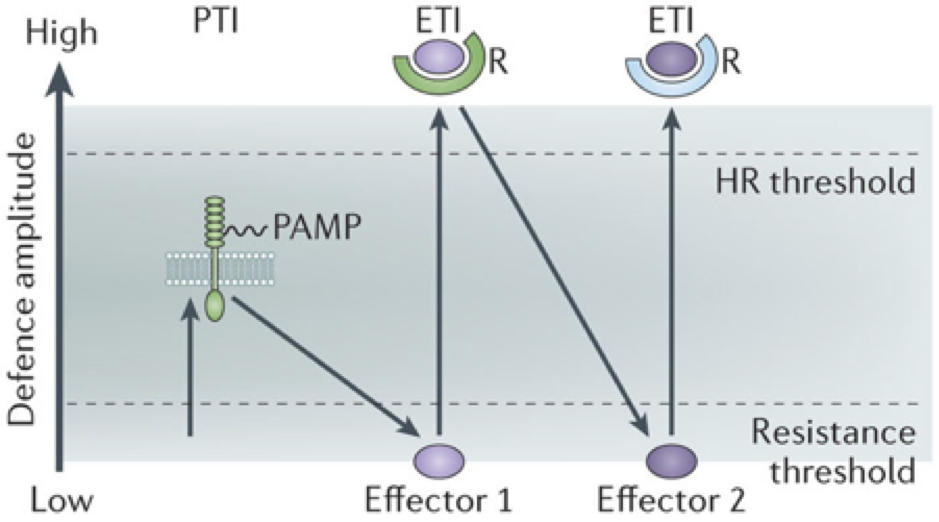
\includegraphics[width=9.78in]{assets/jones_fig1_prac} \caption{The zig-zag model of plant immunity \citep{Jones:2006ih}.
The ultimate amplitude of defence is the combined sum of resistance
output (ETI+PTI) and the difference of the effect of pathogen effectors
(-ETS; effector triggered susceptibility). This diagram captures the
observation that many PTI and ETI outputs are similar, but HR is
associated specifically with successful ETI, and that virulent pathogens
with specific effectors are able to suppress immunity to compromise
immunity. Image is from \citet{Pumplin:2013ix}.}\label{fig:zigzag}
\end{figure}

The aim of this practical session will be to familiarise you with the
use of model organisms to probe the plant immune system. The practical
will include a general introduction to the oomycete pathogens of
Arabidopsis: \emph{Albugo spp} and \emph{Hyaloperonospora arabidopsidis}
(white rust and downy mildew respectively), the bacterial species
\emph{Pseudomonas syringae} and \emph{P. fluorescens}, and the
pathosystem of potato and the oomycete \emph{Phytophthora infestans}
(late blight) (Figure \ref{fig:leaves}).

We will familiarise you with the life cycle, pathogenesis and symptoms
of these pathogens. We will use various techniques to assess the growth
of pathogens on their hosts and to assess immune responses mounted
against these pathogens. For example, we will use light microscopy of
trypan-blue stained Arabidopsis infected with downy mildew to
qualitatively assess the success of infection and resistance of
different genotypes of the pathogen and plant. We will introduce
transient expression systems such as bombardment and \emph{Agrobacterium
tumefaciens}-mediated \emph{Nicotiana tabacum} transformation
(agroinfiltration) to determine the relationship between R- and
avirulence-genes responsible for compatible (resulting in disease) or
incompatible (resulting in healthy plants) interactions.











\begin{figure}
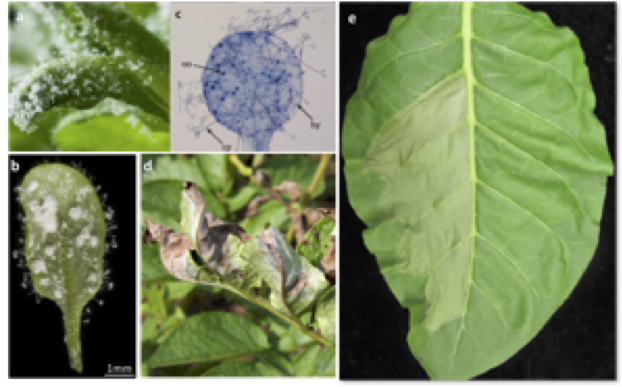
\includegraphics[width=6.48in]{assets/jones_fig2_prac} \caption{Macroscopic characteristics of plant-pathogen
interactions. a, b) Sporulating Hyaloperonospora arabidopsidis (seen on
the edges of the leaf in b) growing on \emph{Arabidopsis thaliana}
leaves. Albugo is also growing on the abaxial surface of the leaf in b.
c) Trypan blue staining of a \emph{H. arabidopsidis-infected} leaf of
Arabidopsis. d) Foliar symptoms of \emph{Phytophthora infestans}
infection of potato. e) Hypersensitive cell death in tobacco leaf
resulting from \emph{Agrobacterium tumefaciens}-mediated transformation
with cognate R gene and Avr gene.}\label{fig:leaves}
\end{figure}

\chapter*{Genomic Resources and Bioinformatics for Plant Microbe
Interactions.}\label{genomic-resources-and-bioinformatics-for-plant-microbe-interactions.}
\addcontentsline{toc}{chapter}{Genomic Resources and Bioinformatics for
Plant Microbe Interactions.}

\textbf{Led by Dan MacLean}

The increase in the generation and analysis of sequence data in the last
ten years has had a profound effect on plant and microbe interaction
research. The genomes of the wide range of host and pathogen's of
interest are now open to study in a way that is within reach of most
scientists - not just large genome sequencing institutes - and many
laboratories are now undertaking genomics as a routine approach.

The deluge of data created by new sequencing approaches has been
collected into a wide range of general and domain specific databases,
each of which contain different information accessed in different ways.
Knowing which are the most useful databases in a given context is
therefore a tricky question and in this session we will take a tour of
the most widely-used including \href{http://ensembl.org}{Ensembl},
\href{http://phytopathdb.org}{PhytoPath},
\href{http://solgenomics.net}{SolGenomics},
\href{http://arabidopsis.org}{TAIR} and
\href{http://araport.org}{AraPort}.

Sequence data are used in a wide range of applications and the source
molecule will be selected in an application specific way. Genomic DNA is
used for assembly of draft genomes, RNA is used for gene expression
analysis, genome annotation and exome construction. Both DNA and RNA get
used to identify genetic polymorphisms. Mixed populations of nucleic
acids from environmental (e.g soil or pathogen/host interaction sites)
are used to study species compositions. A wide range of bioinformatics
tools have been developed and are in common use for these approaches, so
in this topic we will study briefly the tools and their core algorithms
and competencies with the aim of helping you to decide on the right
tools for any particular analysis that you may wish to do outside of the
course. A useful guide is available in \citet{MacLean:2009hm}. In
particular we will look at algorithms and tools for \emph{de novo}
assembly of sequence including SOAPdenovo \citep{Luo:2012fn} and
\href{http://wgs-assembler.sourceforge.net/wiki/index.php?title=Main_Page}{Celera
Assembler}. We will study tools for RNASeq expression and annotation
analyses including Tophat \citep{Trapnell:2009dp} and Bowtie
\citep{Langmead:2012jh} and DESeq \citep{Anders:2010fu} and edgeR
\citep{Robinson:2010cw}.







\begin{figure}
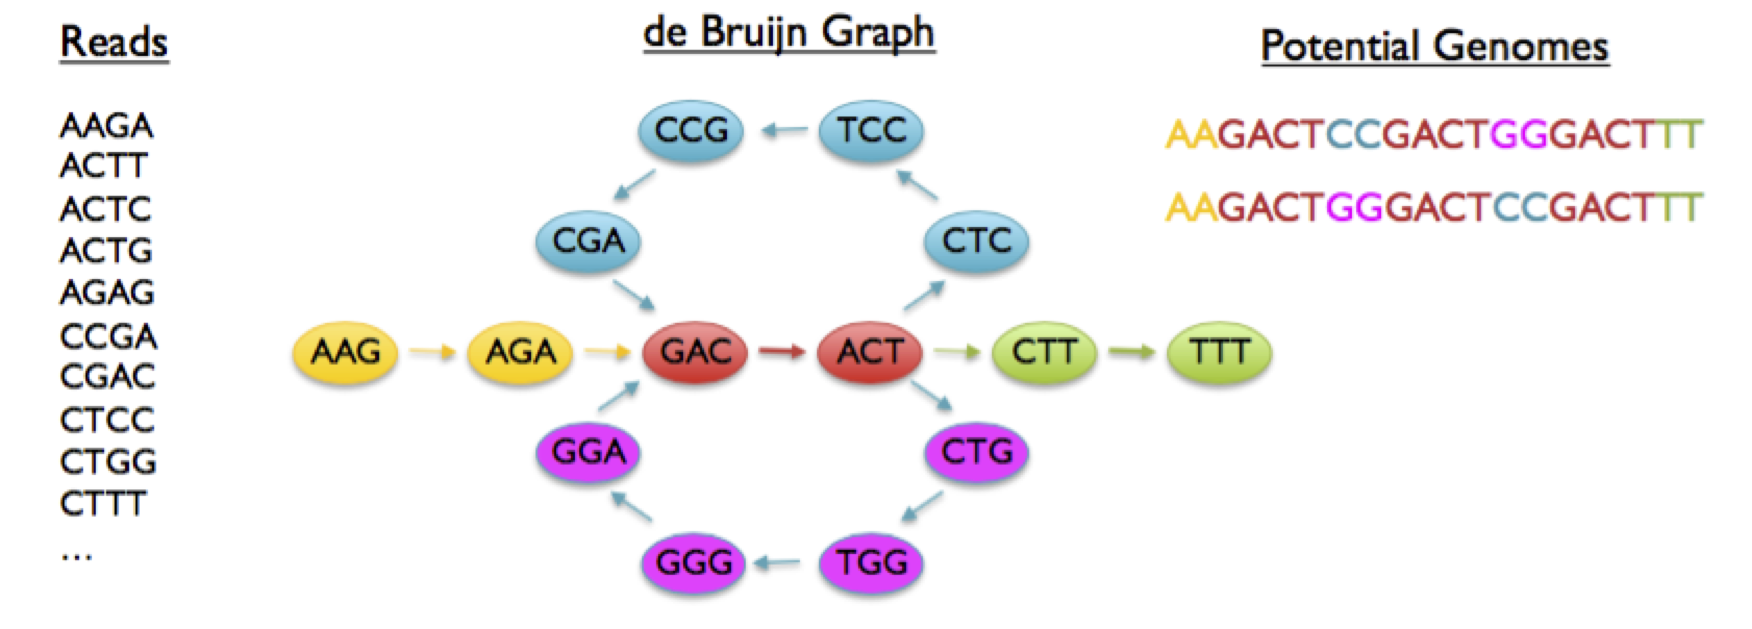
\includegraphics[width=7.01in]{assets/algo} \caption{Graphical summary of a \emph{de novo} assembly algorithm.
Sequence reads are broken down into constituent \emph{k}-mers and a
network of overlapping \emph{k}-mers is produced. The paths in the graph
are traversed and the \emph{k}-mers collected into a growing string
representing a long sequence in the original data and therefore genome.}\label{fig:mainbio}
\end{figure}

\section*{Keynote Lecture}\label{keynote-lecture-1}
\addcontentsline{toc}{section}{Keynote Lecture}

\subsection*{Diane G.O. Saunders - Developing new tools for
interrogating cereal
invaders}\label{diane-g.o.-saunders---developing-new-tools-for-interrogating-cereal-invaders}
\addcontentsline{toc}{subsection}{Diane G.O. Saunders - Developing new
tools for interrogating cereal invaders}

\textbf{John Innes Centre, Norwich, UK}

Emerging and re-emerging pathogens pose a continuous threat to food
security and human health. Recent advances in next-generation sequencing
technologies have provided new opportunities to integrate genomics into
the tracking of emerging filamentous plant pathogens. This approach is
particularly valuable for analysing rust pathogens, which are frequently
obligate biotrophs that cannot be axenically cultured in the laboratory
environment. Accordingly, we are leading the genome sequencing of
hundreds of isolates of the wheat yellow rust pathogen \emph{Puccinia
striiformis f. sp. tritici} (PST), aimed at improving our understanding
of the molecular mechanisms that drive PST evolution. Furthermore, we
have developed a robust and rapid ``field pathogenomics'' strategy to
improve filamentous pathogen surveillance. Using gene sequencing of
PST-infected wheat leaves taken directly from the field, this technique
enabled us to gain insight into the population structure of PST over
successive seasons. Our analysis uncovered a dramatic shift in the PST
population in the UK and supports the hypothesis that a recent
introduction of a diverse set of exotic PST lineages may have displaced
the previous populations. Furthermore, we uncovered potential seasonal
and varietal specificity for specific genotypes of PST. Our discovery of
wheat variety susceptibility to specific \emph{P. striiformis} isolates
that are prevalent at certain times of the year could have considerable
impact on directing future disease management approaches.

\subsection*{About Diane Saunders}\label{about-diane-saunders}
\addcontentsline{toc}{subsection}{About Diane Saunders}

\begin{quote}
Dr.~Saunders received her BSc degree from Exeter University where she
continued her studies to PhD level in the pioneering laboratory of
Prof.~Nick Talbot. After receiving her PhD in 2009 she joined
Prof.~Sophien Kamoun's group at The Sainsbury laboratory (TSL) to
continue to pursue her interest in the molecular mechanisms that
underpin plant-pathogen interactions. Following an early career
Leverhulme fellowship at TSL she was awarded a research fellowship from
the Earlham Institute and the John Innes Centre to develop her own
research group with a focus on emerging and re-emerging plant pathogens.
She was then appointed as Project Leader at the John Innes Centre in
2017 where she continues to pursue a multi-disciplinary approach to her
research, integrating molecular genetics, microbiology, cell biology,
biochemistry, genomics and data mining. In addition, she has worked on
three of the most important plant diseases in the world: rice blast,
potato late blight, and cereal rusts.
\end{quote}

\section*{Practical Session - From Sequence Data to Candidate
Gene}\label{practical-session---from-sequence-data-to-candidate-gene}
\addcontentsline{toc}{section}{Practical Session - From Sequence Data to
Candidate Gene}

\textbf{Led by Dan MacLean}

\subsection*{Aims and Objectives}\label{aims-and-objectives-1}
\addcontentsline{toc}{subsection}{Aims and Objectives}

\begin{enumerate}
\def\labelenumi{\arabic{enumi}.}
\tightlist
\item
  Understand Strengths and Weaknesses of High Throughput Sequence Data
\item
  Know how to call SNPs from HTS data on
\item
  Categorise SNPs according to an expected genetic background
\end{enumerate}

Genomics has come a long way. We can now sequence genomes quickly and to
a reasonable degree of accuracy. We can create in a high-throughput
manner an inventory of sub-regions in a genome that we think are genes.
We know the functions (or some of the functions) of lots of genes and we
can infer functions of newly discovered genes by comparison of sequence
or structure, basically by seeing whether our new thing looks like
something else.

These methods are actually only PREDICTIONS of function. Looking a bit
like something else is only a clue to what something does. It frequently
fails us.

In this practical we will look at the powerful technique of mutational
genomics. This is possibly the coolest thing ever as it involves
mutating a living organism so that it is different from other things and
then sequencing the genome to pinpoint the exact changes that cause the
difference. We don't have the scope or chemicals to do the mutation bit,
so we'll pick up with the genomics and use Galaxy and Galaxy tools to
carry out the analysis that takes us from sequence data to actual
candidate mutations in the genome sequence.

With mutational genomics we deal initially with the effect of the gene
on the whole organism. By performing mutagenesis on our favourite
organism then carrying out a genetic screen \citep{Page:2002ji} that
selects individuals that have changed in the phenotype we are interested
in, we have our first foothold on function. We can study those
individuals and apply the principles of genetics, use modern
high-throughput sequencing and bioinformatics tools to identify the gene
causing that phenotype change (or at least ones involved in the process
we have messed up).

We will use tools in the Galaxy \citep{Goecks:2010ea} framework
including FastQC for quality control of sequence data \citep{FastQC},
BWA for read mapping and alignment \citep{Li:2009fi} and CandiSNP
\citep{Etherington:2014ba} to identify candidate mutations (Figure
\ref{fig:candisnp}) .

\begin{figure}
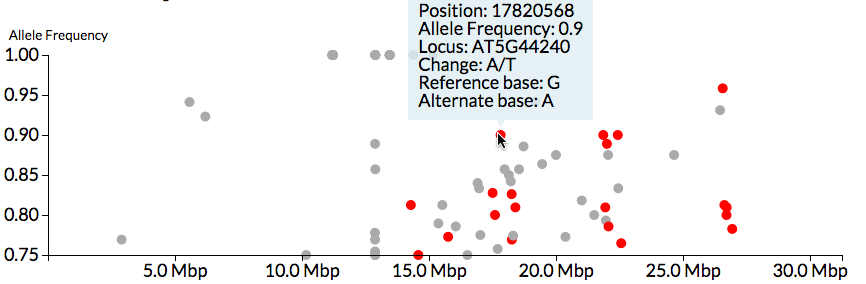
\includegraphics[width=5.77in]{assets/candisnp} \caption{CandiSNP visualisation of SNPs}\label{fig:candisnp}
\end{figure}

\chapter*{Effectors and Immunity}\label{effectors-and-immunity}
\addcontentsline{toc}{chapter}{Effectors and Immunity}

\textbf{Led by Sophien Kamoun}

One of nature's many secrets in biology is how filamentous plant
pathogens cause disease on their hosts. We are making tremendous
progress towards understanding this process largely due to breakthroughs
in ``effector biology'' \citep{Hogenhout:2009em, Win:2012jd}. Effectors
are proteins secreted by pathogens to suppress host immune systems and
manipulate plant physiology to enable pathogen colonization (Figure
\ref{fig:maineff}A).


























\begin{figure}
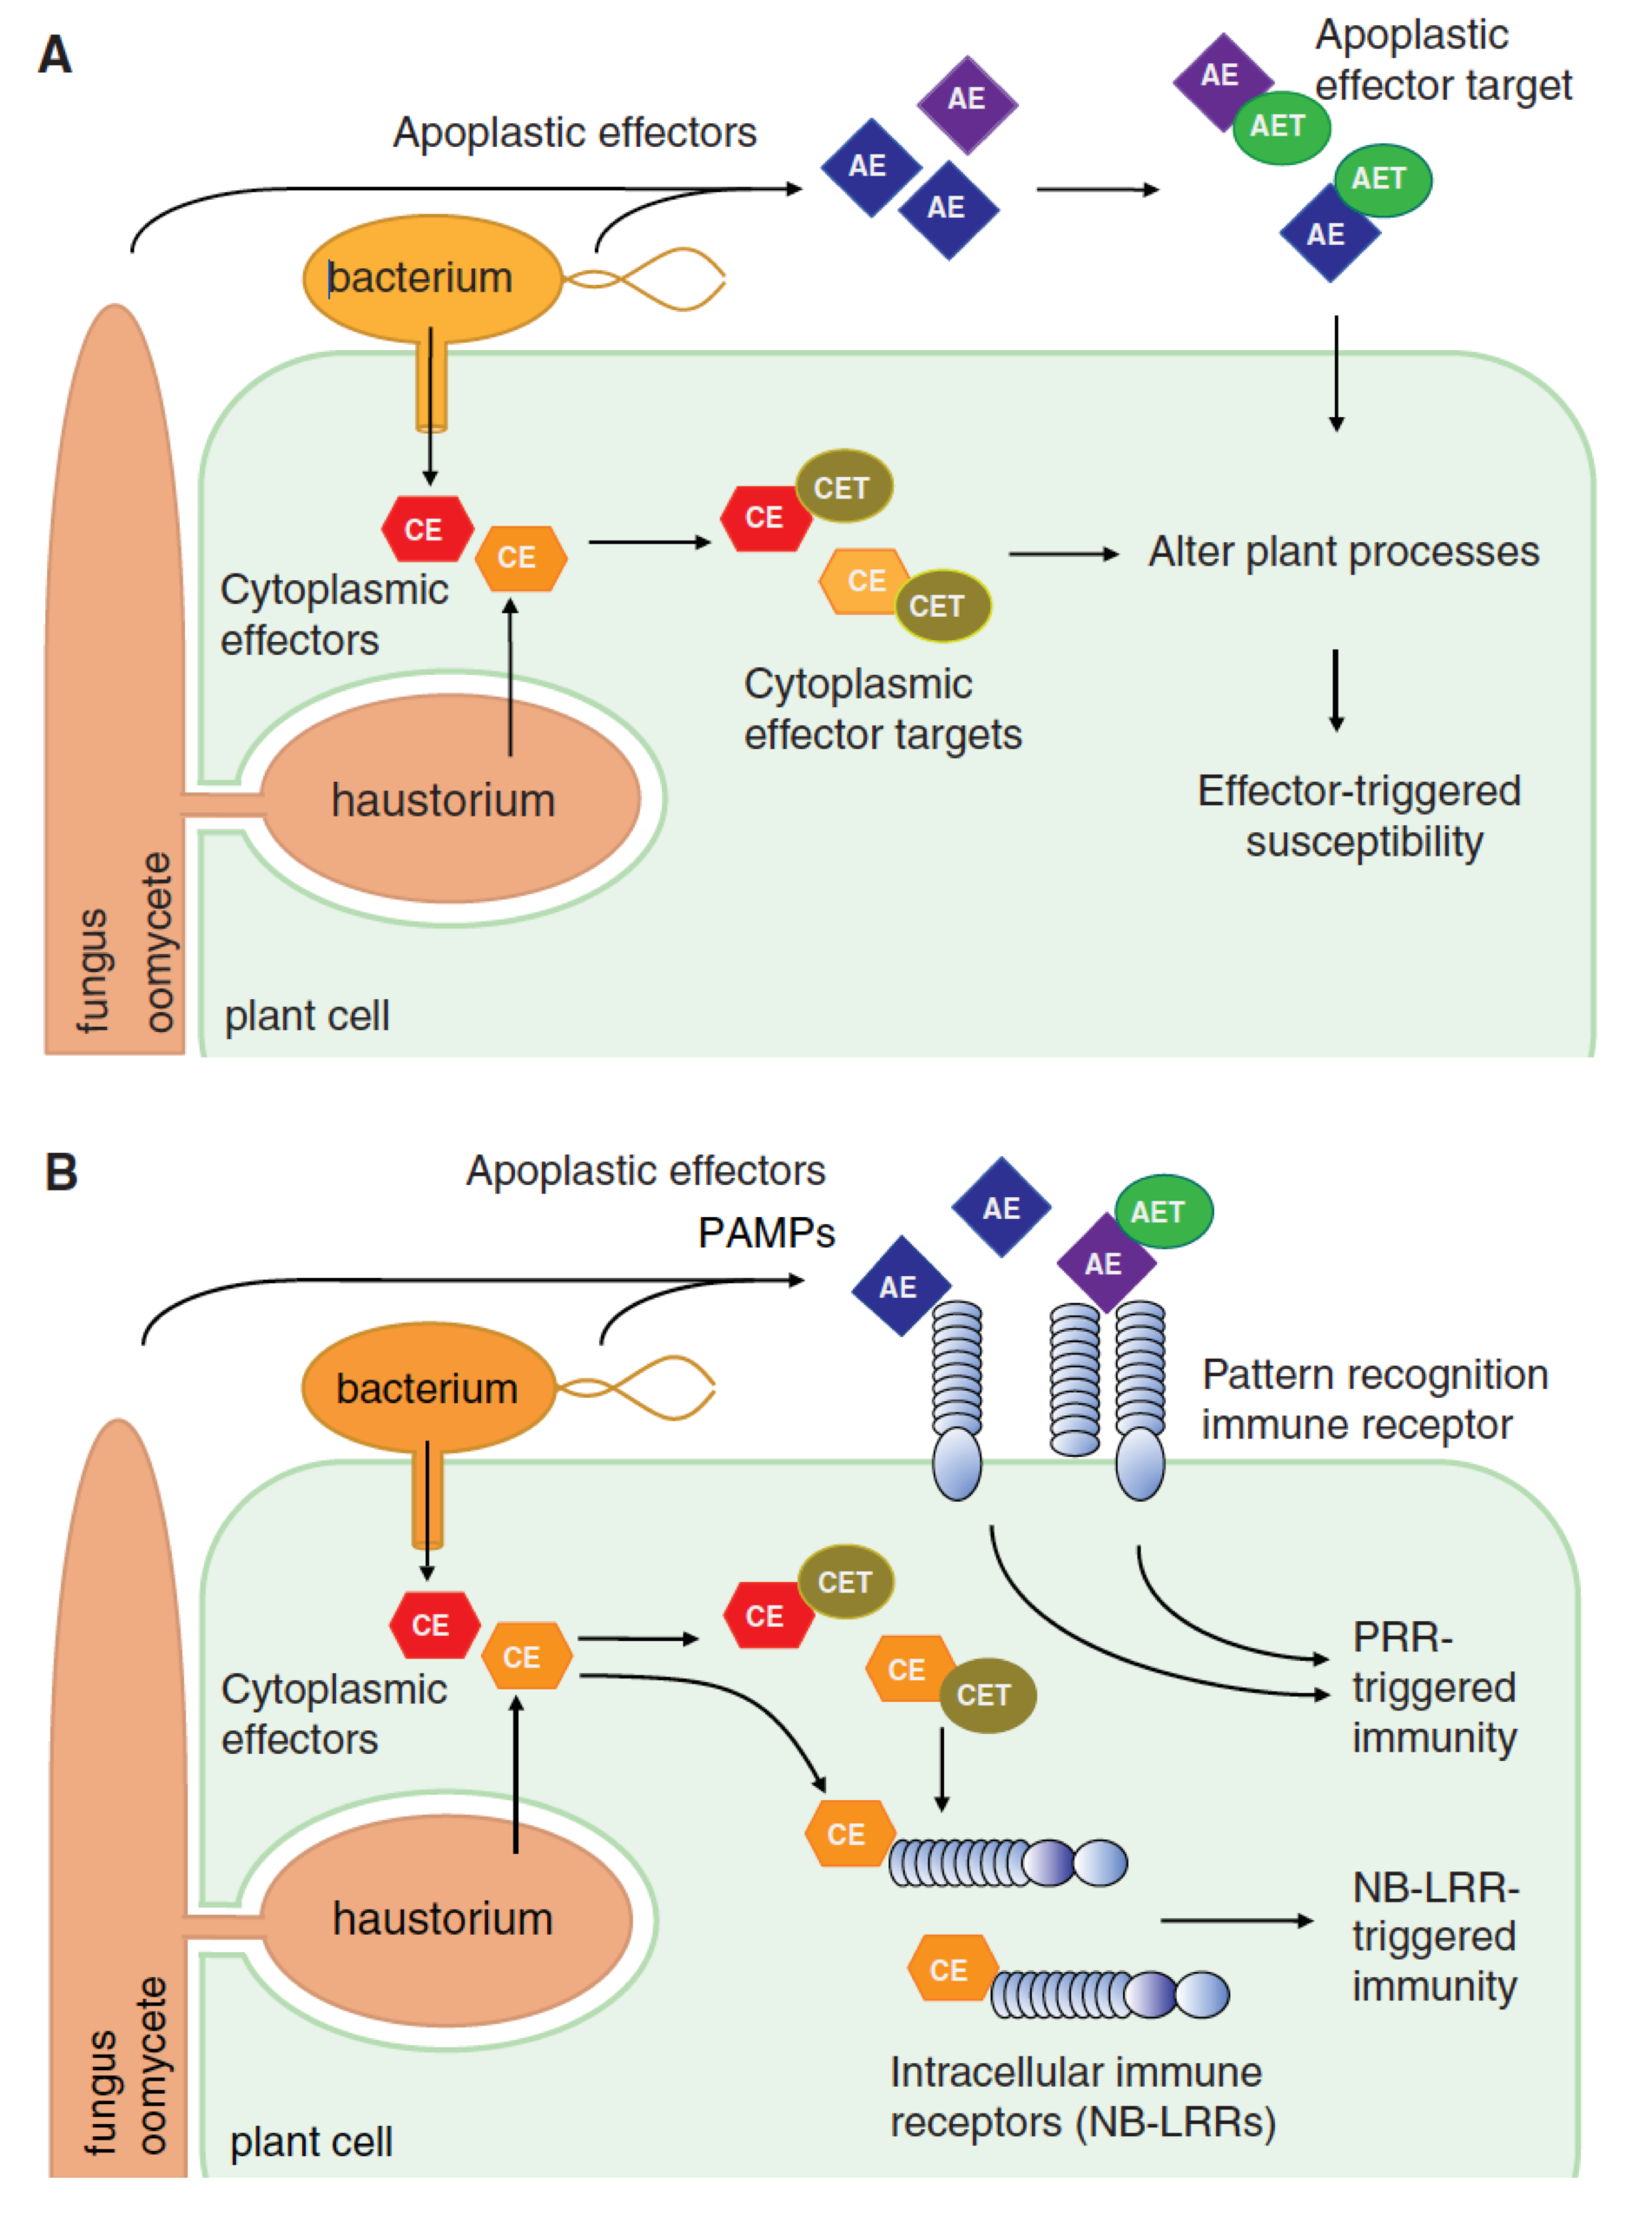
\includegraphics[width=4.75in]{assets/eff} \caption{\textbf{\emph{The concept of effectors in plant immunity}}.
Infectious pathogens such as bacteria, fungi, oomycete, and nematodes
deliver effectors at the interface of the host plant (apoplastic
effectors, AE) or inside the cell (cytoplasmic effectors, CE).
Host-translocated (cytoplasmic) effectors are delivered into the host
cytoplasm through a type-III secretion pilus or specialized infectious
structures called haustoria that form within the cell. Pathogen
effectors traffic to various compartments, bind, and manipulate
different host proteins called targets. Depending on their localization
in the cells, these targets are designated as apoplastic effector target
(AET) and cytoplasmic effector target (CET). Effector--target
interactions impact the outcome of the interaction between the pathogen
and its host. In susceptible genotypes (A), these molecular interactions
can alter plant cell processes and suppress immune responses, leading to
effector-triggered susceptibility (ETS) and host colonization. In
resistant genotypes (B), these interactions are perceived by key sensing
receptors of the immune system that, in turn, stop pathogen growth. Cell
surface pattern recognition receptors (PRRs) detect pathogen-associated
molecular patterns (PAMPs), apoplastic effectors, and/or apoplastic
effector--target interactions to initiate PRRtriggered immunity (PTI).
Intracellular nucleotide-binding receptors (NB-LRR) induce
NB-LRR-triggered immunity (ETI) on recognition of cytoplasmic effectors
and/or cytoplasmic effectors--target interactions (Reproduced from
\citet{Win:2012jd}).}\label{fig:maineff}
\end{figure}

We can predict an ``effectorome'', or effector repertoire, of a pathogen
from its genome sequence based on several criteria that we know about
effectors \citep{Saunders:2012bw}. These criteria include, presence of a
secretory signal peptide, lack of transmembrane domains, lack of
mitochondrial targeting signals, presence of known/conserved motifs such
as RXLR, upregulation of their transcripts during infection, specific
localization in host cells, similarity to known effectors of other plant
pathogen species, etc. However, one persistent question is: What are the
intrinsic functions of these effectors? To find out, we express tagged
effectors in plants and observe their effect on plant morphology and
physiology {[}such as hypersensitive response (HR) cell death{]} using a
technique called the agrobacteria-mediated transient transformation
procedure \citep{Kapila:1997}, also known as agroinfiltration. In
addition, to work out what these effectors might be doing in plants, we
derive clues from the effector-associated plant proteins that we
identify by performing co-immunoprecipitation (co-IP) of tagged
effectors followed by mass spectrometry (MS) \citep{Win:2011dw}. These
plant proteins constitute potential targets of the effectors. We confirm
the association between the effectors and the potential targets in an
independent system known as yeast-two-hybrid interaction assays
\citep{Fields:1989dm}, or in vitro interaction assays. Once we know the
effector targets, we investigate them to find out if they play important
roles in plant-pathogen interactions by knocking down their transcripts
in plants by virus-induced gene silencing (VIGS) \citep{Lindbo:1993kp}
and observing the effects on plant responses to infection.

\pagebreak

\section*{Keynote Lecture}\label{keynote-lecture-2}
\addcontentsline{toc}{section}{Keynote Lecture}

\subsection*{\texorpdfstring{Jens Boch - A battle for life and death -
Evolution of TALEs in plant-pathogenic \emph{Xanthomonas}
bacteria}{Jens Boch - A battle for life and death - Evolution of TALEs in plant-pathogenic Xanthomonas bacteria}}\label{jens-boch---a-battle-for-life-and-death---evolution-of-tales-in-plant-pathogenic-xanthomonas-bacteria}
\addcontentsline{toc}{subsection}{Jens Boch - A battle for life and
death - Evolution of TALEs in plant-pathogenic \emph{Xanthomonas}
bacteria}

\textbf{Leibniz Universität Hannover, Institute of Plant Genetics, 30419
Hannover, Germany}

Plant pathogens embark upon a fierce battle with their plant hosts over
tissue colonization and nutrient acquisition. This has deadly
consequences for both partners of the interaction, but also for us if
crop plants are involved. Plant pathogenic \emph{Xanthomonas oryzae}
bacteria can cause substantial losses in rice, making this pathogen a
key threat to our food production. Like many other plant pathogens,
\emph{Xanthomonas} bacteria translocate a collection of effector
proteins into eukaryotic host cells to function as potent weapons. Among
these effectors, TALEs (transcription activator-like effectors) play a
pivotal role. TALEs act as transcription factors within the plant cell
to induce expression of specific target genes and support the bacterial
infection. The DNA-binding mechanism of TALEs is unique and based on a
number of characteristic 34-amino acid tandem repeats. Each repeat
recognizes one base in the target DNA via one precisely positioned amino
acid of a repeat-variable diresidue (RVD). This modular architecture
allows the rearrangement of TALE repeats to evolve new DNA-binding
specificities matching new virulence targets. Whole genome sequences of
several \emph{Xanthomonas oryzae} strains recently revealed both, the
diversity and conservation of TALEs in \emph{X. oryzae}. In combination
with plant transcript analyses and TALE target prediction we now have an
outstanding opportunity to identify TALE virulence targets and decipher
the pathogen's strategy. The constant evolutionary battle between
pathogen and host has caused evasive mutations in plant promoters that
preclude TALE-binding. Matching modifications in TALEs lead to the
development of aberrant repeats with novel DNA-binding behaviours. This
exemplifies the power of the molecular arms race between pathogen and
host. The simple way of generating any desired DNA-binding specificity
has initiated a worldwide use of TALEs for biotechnological
applications. Designer TALEs and TALE nucleases (TALEN) have
successfully been used for highly efficient genome reprogramming and
genome editing. Today, crops and livestock with novel traits as well as
powerful tools for molecular medicine have already been developed using
TALEs.

Further reading:

\begin{enumerate}
\def\labelenumi{\arabic{enumi}.}
\tightlist
\item
  \citet{Boch:2009fc} Breaking the code of DNA binding specificity of
  TAL-type III effectors.
\item
  \citet{Richter:2014kz} A TAL effector repeat architecture for frame
  shift binding.
\item
  \citet{Grau:2016ft} AnnoTALE: bioinformatics tools for identification,
  annotation, and nomenclature of TALEs from \emph{Xanthomonas} genomic
  sequences
\end{enumerate}

\subsection*{About Jens Boch}\label{about-jens-boch}
\addcontentsline{toc}{subsection}{About Jens Boch}

\begin{quote}
Professor for Plant Biotechnology (2015-present), Leibniz Universität
Hannover, Germany Assistant/Associate Professor (1999-2015), Martin
Luther University Halle-Wittenberg, Germany Postdoctoral Fellow
(1997-1999), Washington University in St.~Louis, USA Postdoctoral Fellow
(1996-1997), MPI for Terrestrial Microbiology, Marburg, Germany Ph.D.
(1996), Philipps University Marburg, Germany
\end{quote}

\section*{\texorpdfstring{Practical Session - Studying Effector Function
\emph{in
planta}}{Practical Session - Studying Effector Function in planta}}\label{practical-session---studying-effector-function-in-planta}
\addcontentsline{toc}{section}{Practical Session - Studying Effector
Function \emph{in planta}}

\textbf{Led by Joe Win}

We are interested in how plants defend themselves against pathogens, and
how the pathogens suppress these defences. Plant immunity is governed by
recognition of effectors by plant immune receptors (Figure
\ref{fig:maineff}B). Once recognized, several signalling processes are
initiated by the receptors and defence is mounted against the invading
pathogen. We have identified a novel network of plant immune components
that is involved in defence signalling of Solanaceous plants
\citep{Wu:2016bio}. We study their function and activities by deploying
the methods such as co-IP, HR assays and VIGS as described above.

In these practical sessions, we will guide you through the techniques
and methods described above to probe plant-microbe interactions with a
focus on effectors and plant immunity.

\subsection*{Aims and Objectives}\label{aims-and-objectives-2}
\addcontentsline{toc}{subsection}{Aims and Objectives}

\begin{enumerate}
\def\labelenumi{\arabic{enumi}.}
\tightlist
\item
  To be familiar with current knowledge of effectors and their roles in
  infection of host plants.
\item
  To understand the roles of helper components in plant immune
  signalling network.
\item
  To understand the theory and practice of methods and techniques that
  are routinely used to study effectors and plant immunity
\end{enumerate}

In this practical session, you will be invited to choose one of the
following techniques for hands-on experience guided by the instructors.

\begin{enumerate}
\def\labelenumi{\arabic{enumi}.}
\tightlist
\item
  In planta co-immunoprecipitation of effectors and associated plant
  proteins, and analysis of effector-plant protein interactions \emph{in
  vitro}
\item
  Yeast two-hybrid assay to study protein-protein interaction
\item
  Agroinfiltration and virus-induced gene silencing to study gene
  functions in plants
\end{enumerate}

\chapter*{Surface Immunity}\label{surface-immunity}
\addcontentsline{toc}{chapter}{Surface Immunity}

\textbf{Led by Cyril Zipfel}

The first layer of plant innate immunity depends on the recognition of
microbes via the perception of pathogen-associated molecular patterns
(PAMPs) or damage-associated molecular patterns (DAMPs) by plasma
membrane-localized pattern recognition receptors (PRRs). Plant PRRs are
ligand-binding receptor kinases or receptor-like proteins that exist in
multi-protein complexes to transduce intracellular immune signaling by
triggering downstream phosphorylation cascades \citep{Couto:2016kq}. The
Arabidopsis leucine-rich repeat receptor kinases (LRR-RKs) FLS2 and EFR
are well-studied PRRs that bind the bacterial PAMPs flagellin and EF-Tu
(or their immunogenic epitopes flg22 and elf18), respectively. In both
cases, ligand-binding triggers rapid hetero-oligomerization with SERK
co-receptors. Of these, BAK1/SERK3 and its closest paralog BKK1/SERK4
are the major regulators of FLS2- and EFR-dependent signaling.
Intriguingly, BAK1 and other SERKs are also involved in various
non-immune signaling pathways \citep{Ma:2016eu}. An allele of
\emph{BAK1} specifically affected in PTI, \emph{bak1-5}, enabled the
uncoupling of BAK1's functions in PTI, brassinosteroid (BR) signaling
and cell death control \citep{Schwessinger:2011ku}, allowing a detailed
characterization of BAK1 in immune signaling without the influence of
the morphological defects observed for other \emph{BAK1} alleles.

The plasma membrane-associated receptor-like cytoplasmic kinase (RLCK)
BIK1 is an immediate convergent substrate of several different PRRs as
well as BAK1 \citep{Couto:2016kq}. In response to PAMP perception, BIK1
is phosphorylated and released from the receptor complex and
subsequently phosphorylates the NADPH oxidase RBOHD, which is required
to produce reactive oxygen species (ROS), one of the first hallmark
responses triggered after PAMP perception
\citep{Kadota:2014bi, Li:2014dx}. Another early PTI response is the
influx of apoplastic Ca\textsuperscript{2+} via yet unknown channels, a
response that is also BIK1-dependent
\citep{Li:2014dx, Ranf:2014fg, Seybold:2014wt}. Subsequently, PAMP
perception results in the activation of MAP kinase cascades and
calcium-dependent protein kinases, which ultimately results in the
transcriptional reprogramming of the cell mostly via WRKY transcription
factors and ultimately to the restriction of pathogen growth
\citep{Couto:2016kq}. Later responses associated with FLS2 and EFR
activation include increased ethylene biosynthesis, callose deposition,
and inhibition of seedling growth \citep{Boller:2009hu}.

\section*{Keynote Lecture}\label{keynote-lecture-3}
\addcontentsline{toc}{section}{Keynote Lecture}

\subsection*{Stefanie Ranf - Specificity of LORE-dependent
lipopolysaccharide immune sensing in
Arabidopsis}\label{stefanie-ranf---specificity-of-lore-dependent-lipopolysaccharide-immune-sensing-in-arabidopsis}
\addcontentsline{toc}{subsection}{Stefanie Ranf - Specificity of
LORE-dependent lipopolysaccharide immune sensing in Arabidopsis}

\textbf{Phytopathology, TUM School of Life Sciences, Technical
University of Munich, Freising-Weihenstephan, Germany}

Innate immunity, triggered upom recognition of microbe-associated
molecular patterns (MAMPs) by specific host receptors, is crucial for
animals and plants. Cell surface components such as lipopolysaccharide
(LPS), peptidoglycan and flagellin are typical MAMPs as they are vital
for microbial survival and common to whole microbial classes. LPS, in
particular the endotoxic lipid~A moiety, of Gram-negative bacteria is
sensed as MAMP in mammals through different extra- and intracellular LPS
receptors. Recently, we found that the receptor-like kinase LORE
(LipoOligosaccharide-specific Reduced Elicitation), which belongs to the
plant-specific class of bulb-type lectin S-domain-1 kinases (SD1-RLKs),
mediates sensitive perception of Pseudomonas LPS in Arabidopsis. The
lipid~A moiety from Pseudomonas LPS alone is sufficient to induce
LORE-dependent immune responses. Interestingly, LORE specifically senses
Pseudomonas and Xanthomonas but not the typical enterobacterial LPS
e.g.~of Escherichia~coli. In mammals, on the contrary, enterobacterial
LPS is the most potent immune activator, whereas Pseudomonas LPS is only
a weak agonist due to structural differences within the lipid~A. Thus,
both mammals and plants evolved to sense LPS via its lipid~A moiety but,
apparently, with distinct epitope specificities and through structurally
unrelated receptors.

\subsection*{About Stefanie Ranf}\label{about-stefanie-ranf}
\addcontentsline{toc}{subsection}{About Stefanie Ranf}

\begin{quote}
Since March 2016 - Independent Emmy-Noether group leader at the
Technical University of Munich, Chair of Phytopathology

Jan. 2013 -- Feb. 2016 - Junior group leader at the Technical University
of Munich, Chair of Phytopathology, Prof.~Dr.~Ralph Hückelhoven

May 2011 -- Dec. 2012 - Postdoctoral research with Prof.~Dr.~Dierk
Scheel and Dr.~Justin Lee, Department of Stress and Developmental
Biology, Institute of Plant Biochemistry (IPB), Halle (Saale)

Jan. 2005 -- Apr. 2011 - Ph.D.~thesis with Prof.~Dr.~Dierk Scheel and
Dr.~Justin Lee, Department of Stress and Developmental Biology,
Institute of Plant Biochemistry (IPB), Halle (Saale)

Oct. 2003 -- Dec. 2004 - Research fellow with Prof.~Dr.~Johannes
Stratmann, University of South Carolina, USA

Oct. 1998 -- Feb. 2003 - Studies of Biochemistry at the Universität
Regensburg
\end{quote}

\newpage

\section*{Practical Session - Analysing Surface
Immunity}\label{practical-session---analysing-surface-immunity}
\addcontentsline{toc}{section}{Practical Session - Analysing Surface
Immunity}

\textbf{Led by Martin Stegmann}

\subsection*{Aims and Objectives}\label{aims-and-objectives-3}
\addcontentsline{toc}{subsection}{Aims and Objectives}

\begin{enumerate}
\def\labelenumi{\arabic{enumi}.}
\tightlist
\item
  Understanding of and hands on experience in classical methods to
  analyse PTI responses in the model organism \emph{Arabidopsis
  thaliana}
\item
  Testing the importance of critical PTI regulators, mainly by analysing
  the impact of PRRs and PRR-associated RLKs on the activation of PTI
  signalling
\item
  Understanding the contribution of PTI on plant immunity against
  adapted bacterial pathogens
\end{enumerate}

The practical session ``Surface Immunity'' will consist of a pedagogical
lecture on the biochemical and molecular biological techniques used to
investigate the molecular basis of PTI signaling, and to identify novel
PAMPs or PRRs. We will demonstrate some of the classical methods used to
analyze downstream PTI responses, such as ROS production, MAPK
activation, seedling growth inhibition and surface immunity upon spray
infection with bacterial pathogens.

For measuring the PAMP-triggered ROS burst, we will make use of a
luminescence-based assay, which enables the detection of apoplastic ROS
that can be monitored live with a charge-coupled device camera. This is
a fast and easy quantitative assay that can be used, in many cases, to
study early PTI signalling in a given mutant compared to a wild type
control.

In addition, we will assay for the induction of a MAPK cascade,
specifically for the PAMP-induced phosphorylation of the four
Arabidopsis MAPKs MPK3, MPK4, MPK6 and MPK11. Their activation can be
detected within a few minutes after PAMP treatment by western blot
analysis using a well-established commercial antibody that was raised to
detect phosphorylated MAPKs in mammalian systems. Prolonged exposure to
PAMPs results in a growth arrest of seedlings, which can be used as a
quantitative measure for the capability of a given genotype to respond
to different stimuli. We will look at different Arabidopsis lines
exposed to PAMPs for several days and assess the resulting growth
differences compared to mock grown seedlings.

Finally, PAMP-triggered immunity contributes to the basal resistance of
plants against adapted pathogens. In the frame of the practical session
we will assess the differences in susceptibility of known PTI pathway
mutants to demonstrate the importance of PTI for plant resistance.

\chapter*{Cellular Defence}\label{cellular-defence}
\addcontentsline{toc}{chapter}{Cellular Defence}

\textbf{Led by Silke Robatzek}

Many microbes that colonize plants invade extracellular spaces. A
physical barrier is thus present between the two organisms. Thus, the
signal exchange between plants and microbes must occur across their cell
surfaces. Pattern recognition receptors (PRRs) are primary sensors of
the plant's immune system, and presented at the plasma membrane to
recognize pathogens and trigger immunity. Recent research has revealed
the machinery that is essential for routing of PRRs and that endocytosis
of PRRs is a mechanism for sustaining cellular responsiveness to confer
long-term anti-bacterial immunity.

The FLAGELLIN SENSING 2 (FLS2) receptor for bacterial flagellin (flg22)
is a prime example to investigate PRR trafficking. Plasma
membrane-localized FLS2 is internalized in a clathrin-dependent manner
and targeted towards distinct subcellular fates in dependence of its
activation status. At the \emph{trans}-Golgi network (TGN),
non-activated FLS2 is recycled back to the plasma membrane. Activated
(flg22-bound) FLS2 is ubiquitinated and sorted into multi-vesicular
bodies (MVBs) of the late endosomal pathway destined for vacuolar
degradation, which is regulated by the endosomal sorting complexes
required for transport (ESCRT) machinery (See Figure \ref{fig:srfig}a).
In light of this, pathogen virulence effectors target TGN-localized
trafficking regulators, and deregulation of the trafficking machinery
i.e.~mutants in clathrin or ESCRT components, enhances infection.

Following recognition of extracellular pathogens by PRRs, defence
components must be delivered across the cell surface to inhibit pathogen
growth. This involves significant reprogramming in secretory and
endocytic trafficking, enabling focal accumulation at infection sites.
Small Rab GTPases and syntaxins act at multiple steps of membrane
trafficking, including cargo selection, vesicle formation, vesicle
movement, tethering and membrane fusion. Distinct members of these
families are associated with specific membrane compartments. Therefore,
these trafficking regulators, i.e.~the Rab5 GTPases ARA6 and ARA7 or the
secretory ARA5 found at the MVB, TGN and Golgi, respectively, represent
molecular probes not only to visualize focal accumulation and PRR
trafficking along the endocytic route, but also to identify
defence-related cargoes that are transported to pathogen infection
sites.

\newpage

\section*{Keynote Lecture}\label{keynote-lecture-4}
\addcontentsline{toc}{section}{Keynote Lecture}

\subsection*{Paul Birch - The Delivery and Activity of late blight
effector proteins that suppress plant
immunity}\label{paul-birch---the-delivery-and-activity-of-late-blight-effector-proteins-that-suppress-plant-immunity}
\addcontentsline{toc}{subsection}{Paul Birch - The Delivery and Activity
of late blight effector proteins that suppress plant immunity}

\textbf{James Hutton Institute, Dundee, UK}

The oomycete Phytophthora infestans causes late blight, the most
significant disease of potato and tomato. As such, it is a threat to
food security. It has been shown to secrete so-called effector proteins
to suppress the host immune system. Some of these effectors, notably the
RXLR class, are delivered (or translocated) inside plant cells where
they interact with host proteins, manipulating their function to promote
disease. We have found that some of these RXLR effectors target and
suppress the activity of plant proteins that are positive regulators of
immunity. In contrast, other RXLRs target negative regulators of
immunity, presumably supporting or promoting their activity to create a
susceptible environment. This presentation will review both classes of
RXLR effector activity, and where this occurs within the plant cell. In
addition, we will look at how these effector proteins are translocated
into the host cell from finger-like structures called haustoria that are
formed by the pathogen during the early stages of infection.

\subsection*{About Paul Birch}\label{about-paul-birch}
\addcontentsline{toc}{subsection}{About Paul Birch}

\begin{quote}
After a PhD and post-doc in University of Manchester on the molecular
biology of lignocellulose degradation by fungi, Paul Birch took up a
Principal Investigator position at the Scottish Crop Research Institute
(now James Hutton Institute) in Dundee in 1995. Since then he has
studied the potato late blight pathogen, Phytophthora infestans, with a
particular interest in the molecular and cellular processes governing
the development of disease or disease resistance. His group has been
instrumental in discovering effector proteins from the pathogen that
enter plant cells and manipulate host defences. In 2007, he became
`Professor of Plant Pathology' at the University of Dundee. In 2016 he
was made Fellow of the Royal Society of Edinburgh. His main interests
are in understanding: • How pathogen effectors are delivered inside
plant cells; • What host proteins and processes they target; • How they
are recognised by host resistance proteins; and • How the complex
co-evolution between host and pathogen dictates the outcomes of
attempted infection.
\end{quote}












\begin{figure}
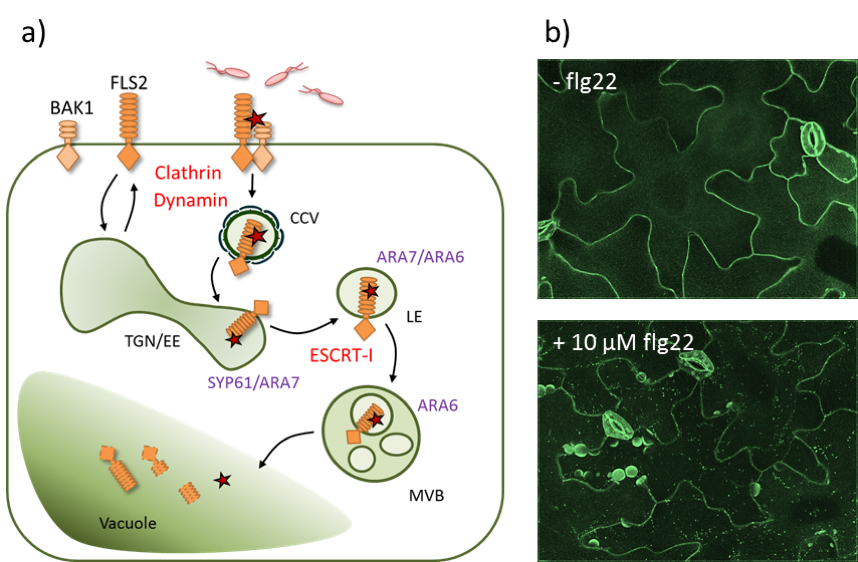
\includegraphics[width=4.9in]{assets/sr_fig1_prac} \caption{FLS2 endocytsosis. \textbf{a)} The PRR FLS2 and its
co-receptor BAK1 localise at the plasma membrane. Upon flg22 perception,
a receptor complex is formed and the activated receptor is internalised
into clathrin-coated vesicles (CCV) and sorted into intraluminal
vesicles of multi-vesicular bodies (MVBs) via the trans-Golgi-network
(TGN)/early endosomes (EE) and the late endosomes (LE). Components
required for FLS2 internalisation and sorting are indicated in red,
endosomal marker proteins are indicated in lilac. \textbf{b)} Confocal
micrographs (spinning disc microscopy) of FLS2-GFP before and after
elicitation with flg22.}\label{fig:srfig}
\end{figure}

\section*{Practical Session - Live Cell Imaging and Investigation of
Subcellular Membrane
Trafficking}\label{practical-session---live-cell-imaging-and-investigation-of-subcellular-membrane-trafficking}
\addcontentsline{toc}{section}{Practical Session - Live Cell Imaging and
Investigation of Subcellular Membrane Trafficking}

\textbf{Led by} \href{gildas.bourdais@sainsbury-laboratory.ac.uk}{Gildas
Bourdais}, \href{michaela.kopischke@sainsbury-laboratory.ac.uk}{Michaela
Kopischke},
\href{agnieszka.siwoszek@sainsbury-laboratory.ac.uk}{Agnieszka
Siwoszek}, \href{jelle.postma@sainsbury-laboratory.ac.uk}{Jelle Postma},
\href{katarzyna.rybak@sainsbury-laboratory.ac.uk}{Katarzyna Rybak},
\href{janina.tamborski@sainsbury-laboratory.ac.uk}{Janina Tamborski}

\subsection*{Aims and Objectives}\label{aims-and-objectives-4}
\addcontentsline{toc}{subsection}{Aims and Objectives}

\begin{enumerate}
\def\labelenumi{\arabic{enumi}.}
\tightlist
\item
  Perform advanced fluorescence imaging using confocal laser scanning
  and spinning disc microscopy
\item
  Generate images suitable for qualitative and quantitative analyses
\item
  Provide a tool-box to understand and study the plant's endomembrane
  trafficking machinery
\end{enumerate}

In the practical sessions we will investigate the (co-)localisation of
FLS2-GFP and various endosomal marker proteins following flg22 treatment
using live-cell imaging approaches (See Figure \ref{fig:srfig} b).
Chemical inhibitors and genetic interference with the endomembrane
trafficking machinery will help us to dissect and understand the route
of activated FLS2 in a temporal and spatial resolution.

\chapter*{Fuctional Plant Genomics}\label{fuctional-plant-genomics}
\addcontentsline{toc}{chapter}{Fuctional Plant Genomics}

\textbf{Led by Ksenia Krasileva}

\emph{Adopting new wheat genomic tools to dissect plant innate immunity}

Almost every week a new plant genome becomes available. Expansion of
genomic data is mostly due to recent advances in sequencing technologies
that have greatly leveraged the field between model and non-model
organisms. Bread wheat (\emph{Triticum aestivum}) is a plant of immense
agronomic value with a highly complex 17 Gb allohexaploid genome. Recent
development of new sequencing and genome assembly approaches greatly
reduced the time and resources needed to assemble wheat genome and 6
genomes of different wheats are already available, allowing for in depth
comparative analyses. Moreover, development of exome capture assay
(targeted sequencing of gene space) allowed establishing reverse
genetics resources for wheat as well as rapid mapping-by-sequencing
identification of mutations from forward genetic screens.

Availability of genome of wheat and many other plant species allowed us
to elucidate evolutionary history of plant immune receptors of
Nucleotide-Binding Leucine Rich Repeat class (NLRs). A recent paradigm
in NLR-based recognition of pathogen derived effectors involves NLRs
with exogenous integrated domains (NLR-IDs) that can serve as baits for
effectors by mimicking plant proteins that pathogens target. We have
shown that NLR-IDs are prevalent across flowering plants and identified
their ID repertoires. This information now allows us to a) search for
new effectors b) predict host susceptibility genes normally targeted by
pathogens (Figure \ref{fig:mainwg}).

\begin{figure}[htbp]
\centering
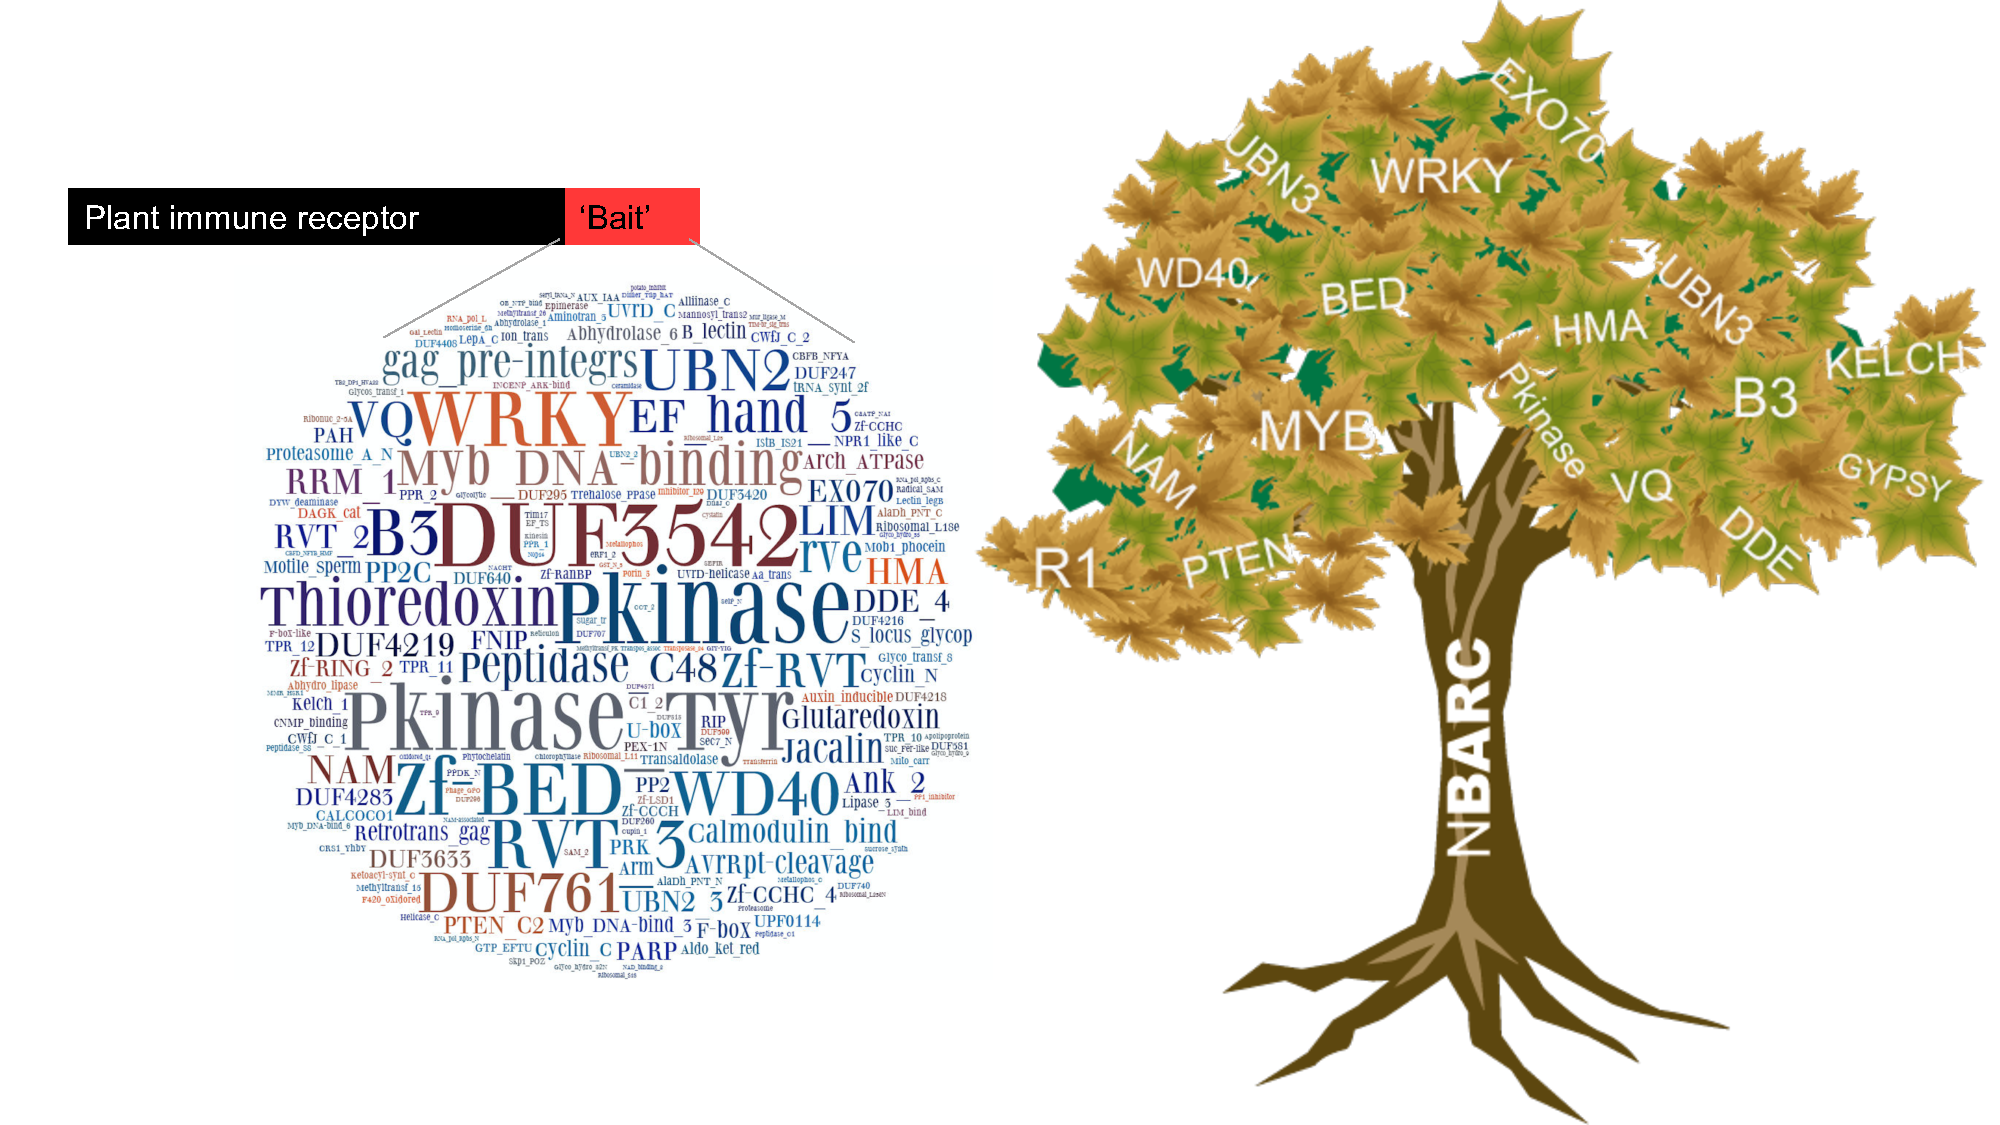
\includegraphics{assets/kk_fig1.pdf}
\caption{\label{fig:mainwg}The NLR Integrated Domain Paradigm}
\end{figure}

\newpage

\section*{Keynote Lecture}\label{keynote-lecture-5}
\addcontentsline{toc}{section}{Keynote Lecture}

\subsection*{Daniel Croll - Retracing genome evolution of pathogens
during rapid disease emergence in agricultural
ecosystems}\label{daniel-croll---retracing-genome-evolution-of-pathogens-during-rapid-disease-emergence-in-agricultural-ecosystems}
\addcontentsline{toc}{subsection}{Daniel Croll - Retracing genome
evolution of pathogens during rapid disease emergence in agricultural
ecosystems}

\textbf{University of Neuchâtel, Switzerland}

Most plants face attacks by pathogens. In agriculture, outbreaks of
fungal diseases are frequent and pose a significant threat to
sustainable food production. What enables pathogens to overcome host
defenses and cause damage is poorly understood. A key evolutionary step
for pathogens is to evolve effectors that specifically target and
disable the plant immune system. We use experimental and population
genomics tools to identify the genes underlying pathogenicity. Our main
model is the fungus \emph{Zymoseptoria tritici}, which causes one of the
most important diseases on wheat. Based on large collections of
sequenced pathogen genomes, we performed genome-wide association studies
(GWAS) to identify the genes linked to the breakdown of host resistance.
These genes encoded small secreted proteins that were highly expressed
during plant infection. Then, we assembled reference-quality genomes to
analyze the chromosomal regions surrounding effector genes. We found
that these regions were undergoing rapid chromosomal sequence evolution
driven by repetitive elements. We found substantial gene deletion
polymorphism segregating in pathogen populations and, hence, functional
differences among pathogen strains. Genes located in highly dynamic
chromosomal regions provide pathogen populations with evolutionary
potential to rapidly adapt to environmental changes or new hosts.

\subsection*{About Daniel Croll}\label{about-daniel-croll}
\addcontentsline{toc}{subsection}{About Daniel Croll}

\begin{quote}
Daniel Croll joined the University of Neuchâtel, Switzerland, in 2017
where he leads the Laboratory of Evolutionary Genetics as an Assistant
Professor. Daniel Croll received his MSc in Biology in 2003 and his PhD
in Life Sciences in 2009 from the University of Lausanne, Switzerland.
He then joined the ETH Zürich as a postdoctoral fellow. Later, he
received an Advanced Postdoctoral Fellowship from the Swiss National
Science Foundation to work 2013-2014 at the University of British
Columbia in Vancouver, Canada. In 2015, Daniel Croll was appointed as an
Oberassistant (group leader) and lecturer at the ETH Zürich. At the
University of Neuchâtel, Daniel Croll continues to investigate the
evolutionary dynamics of disease emergence in agricultural ecosystems.
The main interests include the dissection of phenotypic traits using
genome-wide association mapping, the mechanisms of rapid genome
evolution and the signatures of recent adaptive evolution.
\end{quote}

\newpage

\section*{Practical Session - Functional Plant
Genomics}\label{practical-session---functional-plant-genomics}
\addcontentsline{toc}{section}{Practical Session - Functional Plant
Genomics}

\textbf{Led by Erin Baggs and Elisha Thynne}

\subsection*{Aims and Objectives}\label{aims-and-objectives-5}
\addcontentsline{toc}{subsection}{Aims and Objectives}

\begin{enumerate}
\def\labelenumi{\arabic{enumi}.}
\tightlist
\item
  Become familiar with web-servers and command line tools for protein
  family analyses
\item
  Understand how to produce and critically assess a local sequence
  alignment and phylogeny
\item
  Be able to scan genomes for sequences with particular domains and
  understand their evolutionary origin
\end{enumerate}

The aim of this practical session is to analyse given NLR-IDs as
examples of proteins with complex evolutionary histories and be able to
robustly identify the origins of integrated domains. Each student will
be given an NLR-ID sequences previously identified from our genomic
screens, and will analyse the origin of IDs through genomics and
phylogenetics, predicting what parental gene it might have originated
from. We will also guide you through how to run our r\_gene NLR-ID scan
pipeline (Sarris et al 2016) on a new genome which will allow you to
identify all NLRs and all NLR-IDs from a given proteome. By the end of
the practical we hope you should be able to investigate evolutionary
history of a protein and gain skills in protein family analyses.

The practical will be centred around a biological question of
identifying the origin of integrated domains and predicting parental
genes from which they are derived. The parental genes may in some
instances represent potential pathogen targets, in which are case they
could be considered host susceptibility genes. The practical will be
organized in exercises in different levels to match your skillsets. Our
exercises will take you through the steps of identifying conserved
domains present in a protein of interest and show you how to identify
all sequences in an organism of interest with that domain. Then we will
show you how these sequences can form the basis for an alignment from
which you can generate a phylogeny. At all steps we will highlight
tools, such as BioMart, which will allow you to complete the task with
little bioinformatic skill required. The session will also offer the
chance to use command line tools and scripts available on github which
allow for greater flexibility and control over the data you generate.
The practicals modular composition should allow you to apply many of the
tools introduced to you to your own biological questions.

At the end of the session, we can demonstrate how you can obtain a
knockout of your identified putative susceptibility gene in wheat by
using www.wheat-tilling.com reserse genetics resource.

\chapter*{Application of Discovery and Targeted Proteomics in Plant
Pathogen
Interactions}\label{application-of-discovery-and-targeted-proteomics-in-plant-pathogen-interactions}
\addcontentsline{toc}{chapter}{Application of Discovery and Targeted
Proteomics in Plant Pathogen Interactions}

\textbf{Led by Frank Menke}

The field of proteomics is rapidly advancing, driven in part by
technological innovation and the design of sophisticated approaches to
target a specific biological question. Proteomics is a broad term that
covers the large-scale analysis of proteins and their modifications (the
proteome) in a given cell, tissue or organism under a defined condition.
While this could involve a diverse set of approaches including molecular
biology, biochemistry and genetics, in practise it mostly refers to
protein purification and analysis by mass spectrometry
\citep{Aebersold:2016kt}.

Current developments in the proteomics field are very exciting and
discovery (or shotgun) proteomics data sets are becoming more
comprehensive with more sensitive hybrid mass spectrometers.
Furthermore, targeted proteomics approaches, such as Selective Reaction
Monitoring \citep{Picotti:2013jp} have made it possible to reproducible
and accurately test a biological hypothesis (impossible with shotgun
proteomics at the moment) and bring hands-on proteomics to biologists.

This session will cover the basics of proteomics, including introduction
to mass spectrometry and experimental design. We'll look at both
discovery and targeted proteomic workflows and how these can be used in
studying plant pathogen interactions. See Figure \ref{fig:mainp}.

\section*{Keynote Lecture}\label{keynote-lecture-6}
\addcontentsline{toc}{section}{Keynote Lecture}

\subsection*{Delphine Pflieger - Quantitative phosphoproteomic analysis
reveals shared and specific targets of Arabidopsis MAPkinases MPK3, MPK4
and
MPK6}\label{delphine-pflieger---quantitative-phosphoproteomic-analysis-reveals-shared-and-specific-targets-of-arabidopsis-mapkinases-mpk3-mpk4-and-mpk6}
\addcontentsline{toc}{subsection}{Delphine Pflieger - Quantitative
phosphoproteomic analysis reveals shared and specific targets of
Arabidopsis MAPkinases MPK3, MPK4 and MPK6}

\textbf{Commissariat à l'énergie atomique et aux énergies alternatives
(CEA), Grenoble, France}

In Arabidopsis, mitogen-activated protein kinases MPK3, MPK4 and MPK6
constitute essential relays for a variety of functions including cell
division, development and innate immunity. While some substrates of
MPK3, MPK4 and MPK6 have been identified, the picture is still far from
complete. To identify the substrates of these MAPKs in cell division,
growth and development we compared the cytosolic and chromatin-linked
phosphoproteomes of wild-type and mpk3, mpk4 and mpk6 mutant plants. To
study the function of these MAPKs in innate immunity, we analyzed their
phosphoproteomes following activation by a microbe-associated molecular
pattern (MAMP). We identified 152 differentially phosphorylated peptides
in cytosolic fractions, in response to MAMP treatment and/or when
compared between genotypes. 70 of these could be classified as putative
MAPK targets, with phosphosites that are specific to one or shared by
several MAPKs. Biochemical analysis of a number of putative MAPK
substrates by phosphorylation and interaction assays confirmed our
global phosphoproteome approach. Finally, we examined in detail the
unknown function protein AYL1 (AT5G43830), confirming that it is a MAPK
target and plays a role in defense responses. The results obtained on
the fraction of chromatin-linked phosphoproteins confirm the picture
obtained in the cytosol: in particular, the most dramatic effect on the
phosphoproteome is observed in the mpk6 deletion mutant. In conclusion,
partially overlapping substrate networks were retrieved for all three
MAPKs, showing target specificity to one, two or all three MAPKs in
different biological processes. Interestingly, we unveil the fact that
within a given protein substrate, different phosphosites may be modified
by one specific MAPK or by several of the three MAPKs. Our study also
expands the set of novel MAPK substrates and functions to other involved
protein kinases, including calcium-dependent (CDPK) and sugar
non-fermenting (SnRK) protein kinases.

\subsection*{About Delphine Pflieger}\label{about-delphine-pflieger}
\addcontentsline{toc}{subsection}{About Delphine Pflieger}

\begin{quote}
Delphine Pflieger is a French researcher who followed the boom of
proteomics since the early 2000s, by defending a PhD in 2004 on the use
of the coupling between liquid chromatography and mass spectrometry
(LC-MS) as a very robust and versatile approach for protein sample
characterization. After completing her PhD of Analytical Chemistry in
Paris (University Paris VI), she joined the group of Prof.~Ruedi
Aebersold, starting at the Institute for Systems Biology in Seattle and
then participating in the establishment of a new laboratory in ETH
Zürich. During this post-doctoral experience, she was in particular
interested in developing a proteomics method to better study imperfectly
affinity-purified protein complexes and their phosphorylations. In 2006,
she got a researcher position at CNRS (Centre National de Recherche
Scientifique) in Evry, in the Parisian suburb. In tight collaboration
with the group of Heribert Hirt, she developed there phosphoproteomic
analyses to decipher the signaling cascades triggered in
\emph{Arabidopsis thaliana} when the plant is subjected to a simulation
of pathogen attack. The team analyzed the cytosolic part of the cascades
but also gave a special focus on the events occurring in the vicinity of
chromatin, to connect the very end of the signaling pathways with the
rewiring of the transcriptional program
\citep{Bigeard:2014bl, Bigeard:2014df, Rayapuram:2014dc}. This
collaborative work is still on-going. Since her move to Grenoble in
September 2014, Delphine Pflieger however developed new interests in the
more specific analysis of histones, key constituents of chromatin, both
in terms of variants and of their multiplicity of post-translational
modifications.
\end{quote}

\newpage

\begin{figure}
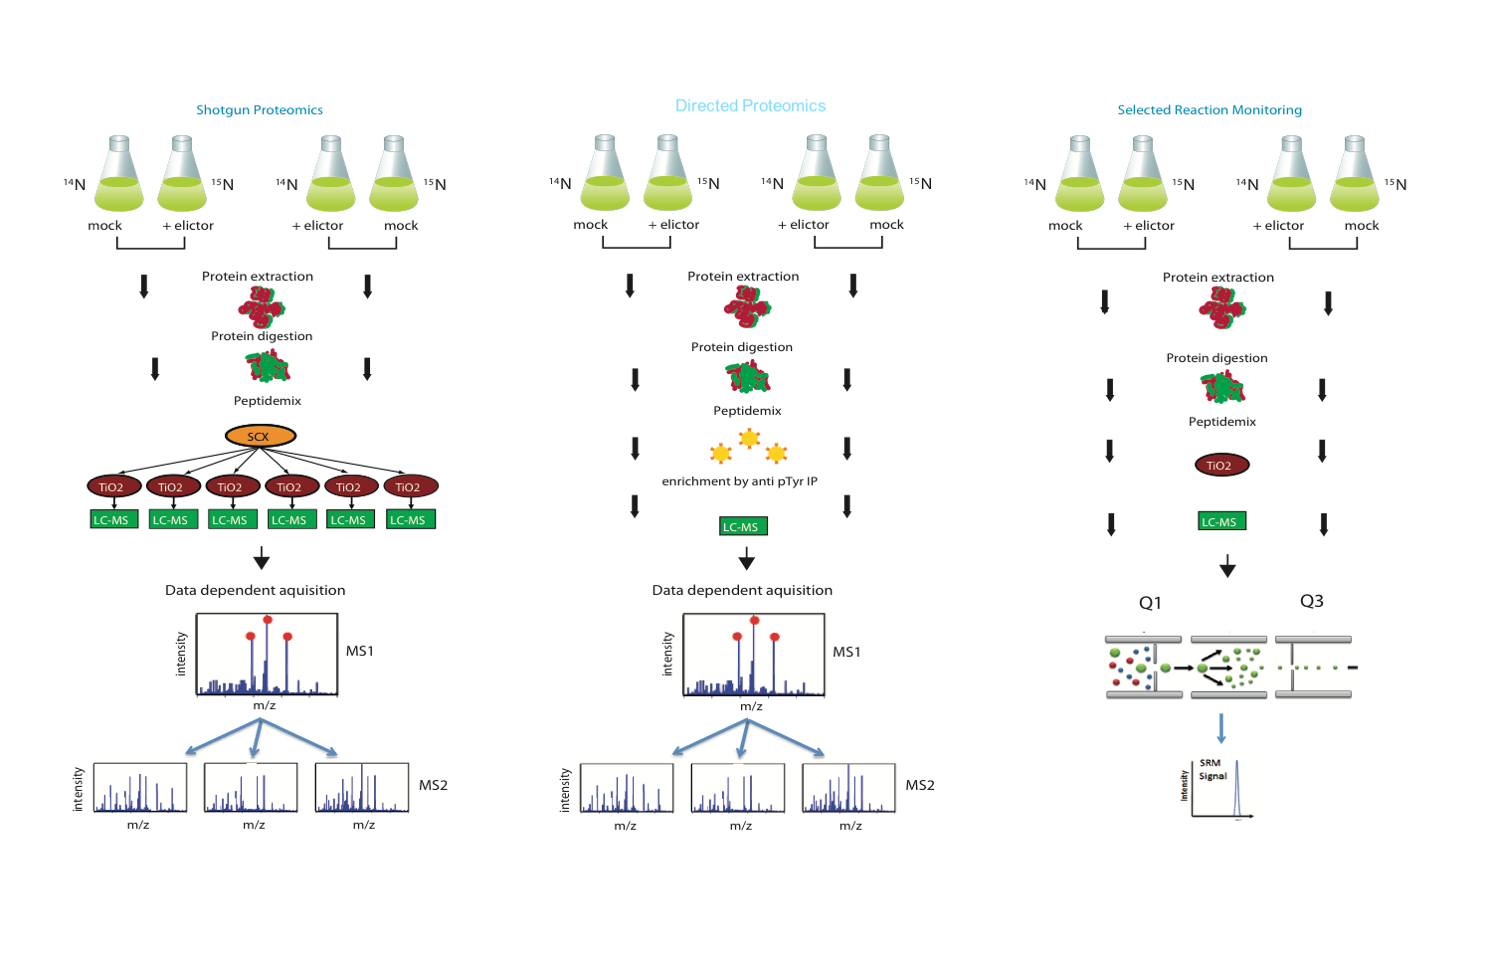
\includegraphics[width=5.97in]{assets/prot1} \caption{Discovery and targets proteomics workflows}\label{fig:mainp}
\end{figure}

\section*{Practical Session - Analysing and interpreting mass spec
data}\label{practical-session---analysing-and-interpreting-mass-spec-data}
\addcontentsline{toc}{section}{Practical Session - Analysing and
interpreting mass spec data}

\textbf{Led by Frank Menke}

\subsection*{Aims and Objectives}\label{aims-and-objectives-6}
\addcontentsline{toc}{subsection}{Aims and Objectives}

\begin{enumerate}
\def\labelenumi{\arabic{enumi}.}
\tightlist
\item
  Understanding how mass spec data analysed
\item
  learning how to interpret targeted proteomics data
\end{enumerate}

Extracting raw data acquired by mass spectrometry to obtain an
interpretable protein list is achieved by step-wise processing of the
data files through a variety of purposely built open source and
commercial software. The first tutorial will cover discovery proteomics
and introduces basic concepts and frequently used data pipelines. Using
actual data collected on TSL mass spectrometers, we will introduce the
most important parameters and variables in data processing, and describe
individual steps of the processing pipeline. We will create textual
input for the search engine, and commence the search to interpret tandem
mass spectra. This will result in a list of identified peptides, their
sequences, and list of proteins. We will then interpret the results
using several software that include web based search engine output,
Scaffold, and data export to tabular format for further processing and
visualization (Figure \ref{fig:pracp} ).

\begin{figure}
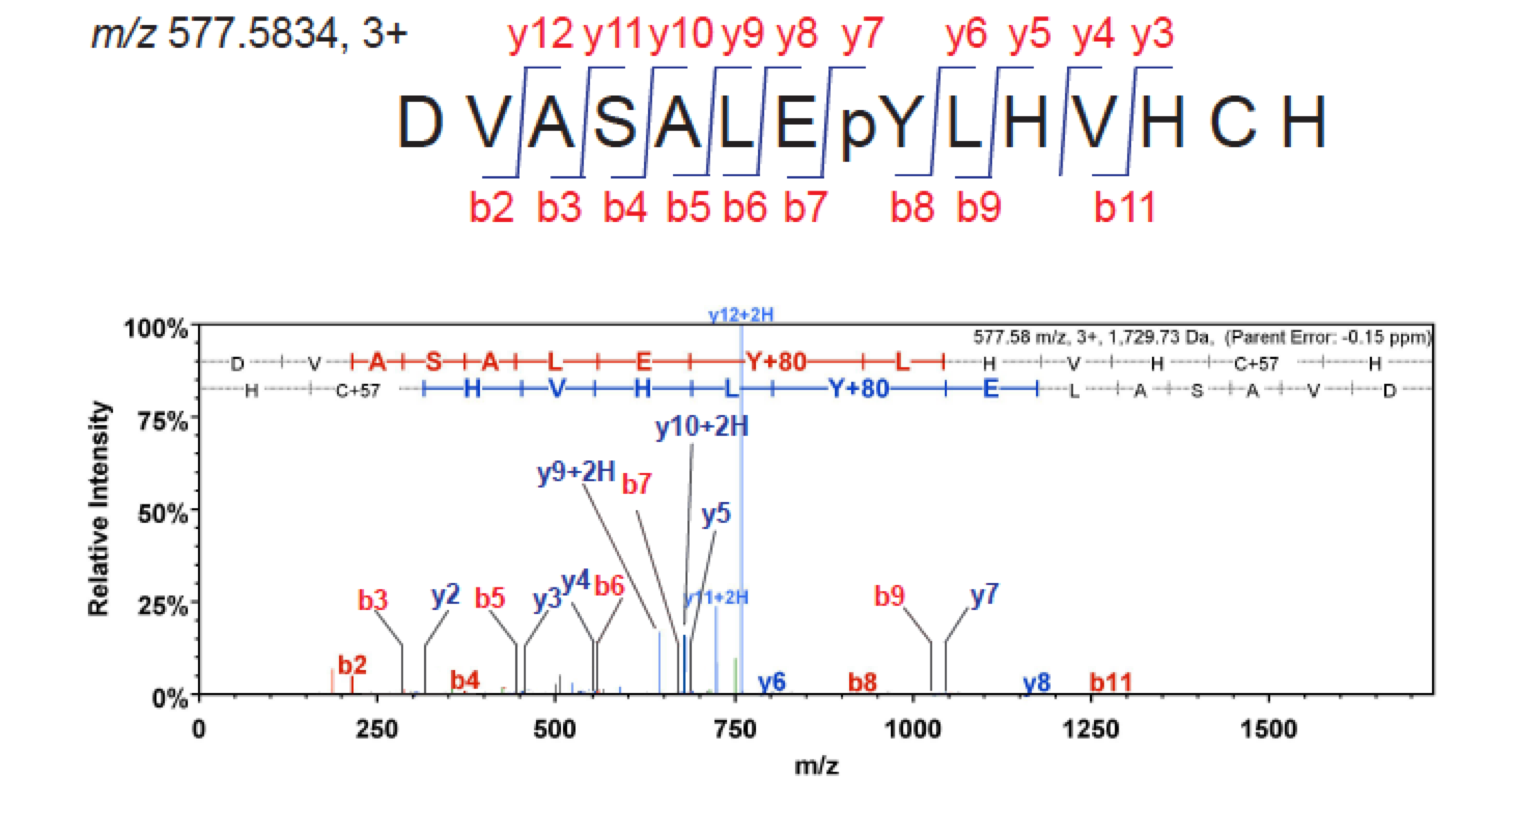
\includegraphics[width=6.06in]{assets/prot2} \caption{Interpretation of a MS2 spectrum}\label{fig:pracp}
\end{figure}

The second tutorial will cover targeted proteomics and analysis of
Selected Reaction Monitoring (SRM) data in Skyline. In this elementary
introduction to Skyline, students will build a spectral library, create
a background proteome, import SRM data files and adjust settings to
allow data refinement, analysis and interpretation.

\chapter*{Translations and Tipping the
Balance}\label{translations-and-tipping-the-balance}
\addcontentsline{toc}{chapter}{Translations and Tipping the Balance}

\textbf{Led by Matt Moscou and Peter Van Esse}

\emph{Exploiting Knowledge of Plant Pathogen Interactions for Durable
Disease Resistance}

In this module we will go into detail about how key insights can be used
to breed and engineer resistant crops and develop durable disease
solutions. We will discuss how pathogen genomics and knowledge of
effectors can lead to an informed deployment of R genes and how effector
biology can be used to accelerate breeding programs. We will discuss
examples where resistance has been transferred between plant species to
introduce novel resistance specificities
\citep{Kawashima:2016hx, Lacombe:2010ga, Tai:1999wa}. We will also
discuss the strengths and weaknesses of classical breeding.

In the first session, we will introduce the current status of
agricultural systems and how our approach to plant breeding effects our
ability to maintain disease resistance. Current approaches rely on
identifying resistance in elite, landrace, and wild cultivars,
identifying markers associated with resistance, and the use of
marker-assisted selection to introduce resistance into elite accessions.
While natural variation has been the primary source of resistance,
pioneering work in nonhost species has paved the way forward for
accessing a broader range of resistance genes for agriculture. We will
discuss how recent technology including high-throughput sequencing,
transformation, gene editing, and synthetic biology will improve our
ability to engineer next-generation crops.

A comprehensive disease management strategy requires a detailed
understanding of the interaction between pathogens and their host or
hosts. As pathogens are diverse, the above outlined strategies require
fine-tuning and rethinking for each individual situation. Novel
incursions are particularly dangerous as they can hit unexpectedly,
spread rapidly, and can cause a great deal of damage long before we can
even begin to understand the pathogen and determine an effective plan of
action. Globalization and climate change are major drivers of new
incursions as habitats of pathogens or their vectors shift. Global trade
and travel enables rapid spread of microbes from one habitat to another.
A rapid identification of a novel pathogen is the first step to mount an
effective and informed response by scientist, breeders and farmers.
After this long term solutions need to be designed and put in place that
require in depth knowledge on plant-pathogen interactions. In the second
session, as a creative exercise, we will work on a long-term solution to
a current disease problem.

In the final part of this module we shall explore how personal
development and career choices can deviate from the classic academic
route. We realize that to successfully meet the challenges faced by
agriculture in the coming years, leaders on all levels and aspects of
agriculture will be required. As scientist are highly educated creative
thinkers they are ideal candidates to take up leadership roles in large
corporations or become successful entrepreneurs in start-up companies.
We believe it is crucial to have the abilities define a career path in
which you can excel and therefore we would like to spend the last
lecture of this summer school on this forward thinking topic. ```

\section*{Keynote Lecture}\label{keynote-lecture-7}
\addcontentsline{toc}{section}{Keynote Lecture}

\subsection*{Beat Keller - Molecular analysis of wheat -- fungal
pathosystems and applications in resistance
breeding}\label{beat-keller---molecular-analysis-of-wheat-fungal-pathosystems-and-applications-in-resistance-breeding}
\addcontentsline{toc}{subsection}{Beat Keller - Molecular analysis of
wheat -- fungal pathosystems and applications in resistance breeding}

\textbf{Department of Plant and Microbial Biology, University of Zürich,
Switzerland}

Several hundred resistance genes against fungal diseases have been
genetically described in the gene pool of wheat and a few of them have
been cloned. The molecular analysis of their origin, diversity and
function has resulted in insight on their evolution and also suggested
better ways for their use in classical as well as molecular breeding.
For example, the discovery of molecular suppressor activities of certain
powdery mildew resistance genes has resulted in a better understanding
of earlier observations in wheat breeding and allows to predict breeding
outcomes. The current focus of our work is on two different aspects of
disease resistance in wheat: first we study the molecular basis of
durable disease resistance and we focus here on the \emph{Lr34} gene
which was originally described as a QTL for durable, quantitative
disease resistance against the fungal pathogen leaf rust. Second, we are
analyzing at the molecular level the interaction of wheat and the fungal
pathogen powdery mildew. This work also includes the identification of
pathogen determinants that are involved in resistance. The new
developments in wheat genomics including the availability of a
high-quality reference genome sequence allow us to develop more
efficient ways to isolate resistance genes. There is a rapidly
increasing number of innovative new approaches to clone genes from the
wheat genome which I will discuss briefly, and we can expect many more
resistance genes being isolated in the near future. The consequences of
these developments for a better use of genetic diversity in wheat
resistance breeding will be discussed. The molecular diversity that has
been revealed by studies on agronomically important resistance genes can
inspire a number of research directions to improve resistance breeding.
For example, natural diversity provides important clues how to engineer
immune receptors for broader recognition spectrum. Furthermore,
modification of gene expression as well as combination of genes using
transgenic approaches has revealed novel ways to improve disease
resistance. Several of these approaches will be presented for the case
of leaf rust and powdery mildew resistance in wheat.

\subsection*{About Beat Keller}\label{about-beat-keller}
\addcontentsline{toc}{subsection}{About Beat Keller}

\begin{quote}
Dr.~Keller received his PhD from the University of Basel, Switzerland,
in 1985, and then was postdoctoral fellow at the Salk Institute for
Biological Studies in La Jolla, San Diego with a long-term fellowship of
the European Molecular Biology Organization. After returning to Europe
he started a research group in collaboration with the wheat breeding
program in Switzerland and became a full professor for Plant Molecular
Biology at the University of Zurich in 1997. The group of Dr.~Keller has
focused on the molecular understanding of fungal disease resistance in
the wheat, maize and barley crop plants. This has resulted in the
molecular identification of a number of agronomically important
resistance genes. More recently, the group has started a large project
on the wheat powdery mildew pathogen to understand resistance at the
molecular level. In addition, fungal pathogenomics is used to study the
evolution of this highly host-specific pathogen. Dr.~Keller was
Vice-president of the Swiss Academy of Sciences from 2000-2006, has led
several large research consortia in Switzerland and was an ERC Advanced
Investigator grant holder from 2010 to 2015. He is a member of the
Research Council of the Swiss National Science Foundation and currently
Head of the Division of Biology at the University of Zurich.
\end{quote}

\section*{Practical Session - QTL
Analysis}\label{practical-session---qtl-analysis}
\addcontentsline{toc}{section}{Practical Session - QTL Analysis}

\textbf{Led by Matt Moscou}

\subsection*{Aims and Objectives}\label{aims-and-objectives-7}
\addcontentsline{toc}{subsection}{Aims and Objectives}

\begin{enumerate}
\def\labelenumi{\arabic{enumi}.}
\tightlist
\item
  Introduction to genetics through practice.
\item
  Introduce basic R packages for QTL analysis, understand how to link
  genotype (genetic maps) with phenotype (continuous/discrete
  measurements) with R/qtl.
\end{enumerate}

\section*{Practical Session - Designing Durable Disease
Solutions}\label{practical-session---designing-durable-disease-solutions}
\addcontentsline{toc}{section}{Practical Session - Designing Durable
Disease Solutions}

\textbf{Led by Peter van Esse}

\subsection*{Aims and Objectives}\label{aims-and-objectives-8}
\addcontentsline{toc}{subsection}{Aims and Objectives}

\begin{enumerate}
\def\labelenumi{\arabic{enumi}.}
\tightlist
\item
  Familiarize ourselves with lateral thinking
\item
  Brainstorm on potential solutions for a current disease problem in
  agriculture
\end{enumerate}

\subsubsection*{Further Reading}\label{further-reading}
\addcontentsline{toc}{subsubsection}{Further Reading}

The impact of crop protection on agricultural production,
\citet{Popp:102401}

Mendel's laws of inheritance and wheat breeding, \citet{biffen_1905}

Pathogen population genetics, evolutionary potential, and durable
resistance, \citet{McDonald:2002da}

\chapter*{General Information}\label{general-information}
\addcontentsline{toc}{chapter}{General Information}

\section*{Arriving into Norwich}\label{arriving-into-norwich}
\addcontentsline{toc}{section}{Arriving into Norwich}

\subsection*{Arriving by Air}\label{arriving-by-air}
\addcontentsline{toc}{subsection}{Arriving by Air}

\textbf{Norwich International Airport}

\href{http://www.norwichairport.co.uk/}{Norwich International Airport}
is served by \href{http://www.klm.com/}{KLM} and the regional carriers
\href{http://www.flybe.com/}{Flybe},
\href{http://www.bmiregional.com/}{BMI Regional}, and
\href{http://www.easternairways.com/}{Eastern Airways}, with direct
connections to Amsterdam, Manchester, Edinburgh, and Aberdeen. Form the
airport you can take a taxi or
\href{http://www.travelineeastanglia.org.uk/ea/XSLT_TTB_REQUEST?language=en\&command=direct\&net=ea\&line=21603\&sup=\%20\&project=y08\&outputFormat=0\&itdLPxx_displayHeader=false\&lineVer=1\&itdLPxx_spTr=1}{local
bus} (with transfer) to get to the Norwich Research Park. Note that if
you fly out of Norwich airport you will need to pay a
\href{http://www.norwichairport.co.uk/content.asp?pid=92}{£10 Airport
Development Fee} before you can go to your gate. Norwich airport is,
however, a very convenient way to reach Norwich from outside the UK.

\textbf{London Airports}

You can also arrive at any of the London airports and take a train or
coach to Norwich. Stansted Airport is the closest and has direct rail
connections to Norwich.

\subsection*{Arriving by Train}\label{arriving-by-train}
\addcontentsline{toc}{subsection}{Arriving by Train}

Another option, especially if you are based in the UK, or are arriving
at another airport, it to take Britain's national train network to
\href{http://www.nationalrail.co.uk/stations_destinations/NRW.aspx}{Norwich
Train Station}, located in downtown Norwich. From there you can take a
local bus or a taxi to Norwich Research Park.
\href{http://www.nationalrail.co.uk/}{National Rail} and
\href{http://www.thetrainline.com/stations/norwich}{TheTrainLine} are
two comprehensive online resource for booking train travel within the
UK.

\subsection*{Arriving by Coach}\label{arriving-by-coach}
\addcontentsline{toc}{subsection}{Arriving by Coach}

You can also arrive in Norwich via coach.
\href{http://www.norfolk.gov.uk/Travel_and_transport/TravelNorfolk/Buses/Bus_interchanges_and_stops/NCC155388}{Norwich
Bus Station} is downtown and is also served by local buses and taxis
once you arrive.

\subsection*{Arriving by Car and
Parking}\label{arriving-by-car-and-parking}
\addcontentsline{toc}{subsection}{Arriving by Car and Parking}

See the \href{http://www.tsl.ac.uk/contact/}{Sainsbury Laboratory} and
\href{https://www.uea.ac.uk/about/visiting-staying/getting-here}{UEA}
\emph{getting here} pages.

Parking at the Conference Centre is
``\href{http://www.venue-norwich.info/FAQs.html}{ample and free for all
events}''. If you require parking at the conference venue, please use
the JIC Visitor's car park (follow the signs we will put up). When you
are at registration, please tell us your license plate number, make, and
colour so we can register it with JIC security.

Those staying at UEA will be able to park in the Main car park on
campus. Parking will be available in the Main car park on campus. UEA
car park charges are listed on the
\href{https://portal.uea.ac.uk/estates/travel-and-transport/by-car/parking-for-visitors}{UEA
car parking for visitors} page

\subsection*{Getting from and into Central Norwich by
Bus}\label{getting-from-and-into-central-norwich-by-bus}
\addcontentsline{toc}{subsection}{Getting from and into Central Norwich
by Bus}

\href{http://www.firstgroup.com/ukbus/suffolk_norfolk/journey_planning/maps/}{First
Group} is the major local bus provider in Norwich.
\href{http://www.firstgroup.com/ukbus/suffolk_norfolk/assets/pdfs/journey_planning/maps/norwich_map.pdf}{This
map shows the complete network}, and these buses specifically serve the
Norwich Research Park or the UEA campus:

\begin{itemize}
\tightlist
\item
  \textbf{\href{https://www.firstgroup.com/norfolk-suffolk/plan-journey/timetables/?operator=22\&service=11/12\&page=1\&redirect=no}{11/12}}:
  Can catch these routes by walking down Colney Lane, towards the
  Hospital, and at the first bus stop past the roundabout.
\item
  \textbf{\href{https://www.firstgroup.com/norfolk-suffolk/plan-journey/timetables/?operator=22\&service=13/13A/13B/13C/X13\&page=1\&redirect=no}{13/13A/13B/13C/X13}}:
  Can catch these routes by walking down Colney Lane, towards the
  Hospital, and at the first bus stop past the roundabout.
\item
  \textbf{\href{https://www.firstgroup.com/norfolk-suffolk/plan-journey/timetables/?operator=22\&service=21\&page=1\&redirect=no}{21/21A/22}}:
  Can catch these right outside Norwich Research Park, on Colney Lane.
\item
  \textbf{\href{https://www.firstgroup.com/norfolk-suffolk/plan-journey/timetables/?operator=22\&service=25\&page=1\&redirect=no}{25}}:
  Goes from the rail station through the UEA campus, all the way to the
  end of Chancellor's Drive.
\item
  \textbf{\href{http://www.firstgroup.com/ukbus/suffolk_norfolk/journey_planning/timetables/index.php?operator=22\&service=26\&page=1\&redirect=no}{26/26A}}:
  Goes from the rail station to University and nearby hospital. Can
  catch the 26 right out Norwich Research Park, on Colney Lane.
\item
  These bus stops have been added to the
  \href{https://drive.google.com/open?id=1z7gP4EFxyaGBmp69A2woREZWNj0\&usp=sharing}{Summer
  School Google Map}.
\end{itemize}

\section*{Checking into Accomodation}\label{checking-into-accomodation}
\addcontentsline{toc}{section}{Checking into Accomodation}

Accommodation will be at the UEA, Britten House. Check in will be at the
UEA Security Lodge at any time from 2pm on the day of your arrival.

\section*{Meals}\label{meals}
\addcontentsline{toc}{section}{Meals}

\subsection*{Breakfast and Lunch}\label{breakfast-and-lunch}
\addcontentsline{toc}{subsection}{Breakfast and Lunch}

Breakfast in the Zest Restaurant is served each day from 8 am to 9 am.
Lunches can be purchased from The Centrum building on site, a range of
salads, sandwiches, soups and hot meals are available. Coffee, tea and
other beverages will be available during breaks.

\subsection*{Evening Meals}\label{evening-meals}
\addcontentsline{toc}{subsection}{Evening Meals}

Evening meals are self catered. The official conference dinner is on
Friday 4th August.

\subsubsection*{Dining Out}\label{dining-out}
\addcontentsline{toc}{subsubsection}{Dining Out}

Norwich is a compact, walkable city with abundant restaurants and cafes.
Head to either Rampant Horse Street area, The Lanes, or the Tombland
area.

UEA Restaurant facilities on campus provide everything from a simple
coffee and sandwich to a full meal at eateries Blend, Zest, Vista, Café
Direct, Cafe 57 and the Sainsbury Centre for Visual Arts Gallery Café,
though these have restricted opening times, usually until 8pm only and
especially outside of terms.

\subsubsection*{Dining In}\label{dining-in}
\addcontentsline{toc}{subsubsection}{Dining In}

The lodging buildings each have a shared kitchen and you will be able to
prepare small meals there. There is a small supermarket on site in the
main plaza, a short walk from the lodging. There are also three
supermarkets just off campus and within walking distance. These are
marked on the included map.

\section*{Getting Around}\label{getting-around}
\addcontentsline{toc}{section}{Getting Around}

Lodging is at The University of East Anglia, in Britten House. Parking
is available in the main campus car park. There is a custom Google Map
with all venues and Norwich Airport and train and bus stations:
\href{https://drive.google.com/open?id=1z7gP4EFxyaGBmp69A2woREZWNj0\&usp=sharing}{Summer
School Map}

\section*{Site Registration}\label{site-registration}
\addcontentsline{toc}{section}{Site Registration}

On the first morning of The Summer School, please go to the John Innes
Centre Reception for 10 am. We can then sign you into the register
on-site and show you to the training rooms.

\section*{Emergency Contacts}\label{emergency-contacts}
\addcontentsline{toc}{section}{Emergency Contacts}

\subsection*{Internal Emergency First
Aid}\label{internal-emergency-first-aid}
\addcontentsline{toc}{subsection}{Internal Emergency First Aid}

Dial \textbf{333}, ask operator for a First Aider or an ambulance. Or
dial \textbf{9 999} for emergency services directly.

\subsection*{Hospital}\label{hospital}
\addcontentsline{toc}{subsection}{Hospital}

The Norfolk and Norwich University Hospital is directly located on the
Norwich Research Park: Colney Lane, Norwich, NR4 7UY. Tel: 01603 286286.

\section*{Transport}\label{transport}
\addcontentsline{toc}{section}{Transport}

\begin{itemize}
\tightlist
\item
  Taxis -- Goldstar Taxis 01603 700700 or ABC Taxis 01603 666333
\item
  Bus - First Group is the major local bus provider in Norwich and these
  buses specifically serve the Norwich Research Park or the UEA campus:
\item
  \textbf{\href{https://www.firstgroup.com/norfolk-suffolk/plan-journey/timetables/?operator=22\&service=11/12\&page=1\&redirect=no}{11/12}}:
  Can catch these routes by walking down Colney Lane, towards the
  Hospital, and at the first bus stop past the roundabout.
\item
  \textbf{\href{https://www.firstgroup.com/norfolk-suffolk/plan-journey/timetables/?operator=22\&service=13/13A/13B/13C/X13\&page=1\&redirect=no}{13/13A/13B/13C/X13}}:
  Can catch these routes by walking down Colney Lane, towards the
  Hospital, and at the first bus stop past the roundabout.
\item
  \textbf{\href{https://www.firstgroup.com/norfolk-suffolk/plan-journey/timetables/?operator=22\&service=21\&page=1\&redirect=no}{21/21A/22}}:
  Can catch these right outside Norwich Research Park, on Colney Lane.
\item
  \textbf{\href{https://www.firstgroup.com/norfolk-suffolk/plan-journey/timetables/?operator=22\&service=25\&page=1\&redirect=no}{25}}:
  Goes from the rail station through the UEA campus, all the way to the
  end of Chancellor's Drive.
\item
  \textbf{\href{http://www.firstgroup.com/ukbus/suffolk_norfolk/journey_planning/timetables/index.php?operator=22\&service=26\&page=1\&redirect=no}{26/26A}}:
  Goes from the rail station to University and nearby hospital. Can
  catch the 26 right out Norwich Research Park, on Colney Lane.
\end{itemize}

These bus stops have been added to the
\href{https://drive.google.com/open?id=1z7gP4EFxyaGBmp69A2woREZWNj0\&usp=sharing}{Summer
School Google Map}.

\section*{Norwich and Norwich Research
Park}\label{norwich-and-norwich-research-park}
\addcontentsline{toc}{section}{Norwich and Norwich Research Park}

At the heart of East Anglia Norwich is a vibrant inviting city. Steeped
in historic charm; The Cathedral, The Castle, the most complete medieval
street pattern in the UK, the largest collection of pre-reformation
churches in Northern Europe and the oldest hotel in the UK are all
situated in Norwich. In medieval times Norwich was the second largest
city in England. Norwich has the largest open-air market in England plus
its own mustard ``Colmans mustard'' and Norwich City Football Club, The
Canaries. In 2012 Norwich became a UNESCO city of literature. Norwich
has a fantastic surrounding countryside including the Broads and Norfolk
coast.

The Norwich Research Park, with six independent partner institutions;
UEA, The John Innes Centre, Earlham Institute, Quadram Institute,
Norfolk and Norwich Hospital and The Sainsbury Laboratory. Norwich
Research Park is ranked fourth in the UK for the number of
internationally recognised scientists. UEA has the second highest
graduate retention rate in the country with almost half of all graduates
living and working locally.

\section*{Wifi Connections}\label{wifi-connections}
\addcontentsline{toc}{section}{Wifi Connections}

Wifi is available throughout the site. If you have EDUROAM available,
please use that. If you don't have EDUROAM, you can get guest wireless
passes from The John Innes Centre Reception.

\section*{Social Media}\label{social-media}
\addcontentsline{toc}{section}{Social Media}

Tweeting and other social media activity are encouraged.
\texttt{\#tslsummerschool}, \texttt{@TheSainsburyLab}

\section*{Map}\label{map}
\addcontentsline{toc}{section}{Map}

A live Google Map with useful sites marked is available
\href{https://drive.google.com/open?id=1z7gP4EFxyaGBmp69A2woREZWNj0\&usp=sharing}{here}

A static version is presented below.

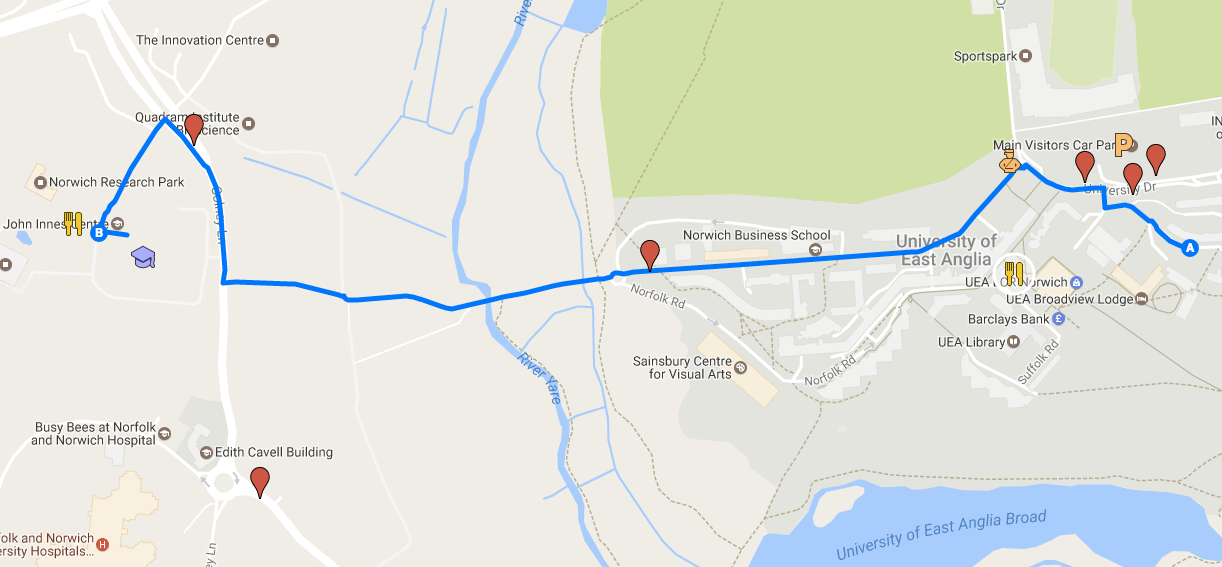
\includegraphics[width=6.11in]{assets/large_map}

\section*{Excursion}\label{excursion}
\addcontentsline{toc}{section}{Excursion}

Sunday is a day of relaxation and we have booked a trip to the north
Norfolk coastal town of Cromer. Perched on the very edge of the north
Norfolk coast, Cromer is famous for its tasty crabs, wide open beaches,
a traditional pier complete with a theatre providing seaside special
variety shows and is awash with small local independent shops. The town
offers a wide choice of restaurants and cafes with not a single coffee
shop chain or national eating or drinking venue to be found. Instead you
have cafes, bars and restaurants owned and operated by local residents
all eager to serve both local residents and visiting guests. The bus
will depart at 1100 am from John Innes Reception.

Later in the day, we have booked a boat in the nearby village of Morston
to take us for a 1 hour trip out on Blakeney Point to see the population
of seals that live there. The boat will leave at 16:45 and the bus will
drop off at Morston from Cromer.

Your hosts for this trip will be Karen Smith and Janina Tamborski,
valuable members of TSL. They'll be around to co-ordinate logistics on
the day.

\bibliography{packages.bib,book.bib,res.bib}


\end{document}
